\documentclass{book}
\usepackage[a4paper,top=2.5cm,bottom=2.5cm,left=2.5cm,right=2.5cm]{geometry}
\usepackage{makeidx}
\usepackage{natbib}
\usepackage{graphicx}
\usepackage{multicol}
\usepackage{float}
\usepackage{listings}
\usepackage{color}
\usepackage{ifthen}
\usepackage[table]{xcolor}
\usepackage{textcomp}
\usepackage{alltt}
\usepackage{ifpdf}
\ifpdf
\usepackage[pdftex,
            pagebackref=true,
            colorlinks=true,
            linkcolor=blue,
            unicode
           ]{hyperref}
\else
\usepackage[ps2pdf,
            pagebackref=true,
            colorlinks=true,
            linkcolor=blue,
            unicode
           ]{hyperref}
\usepackage{pspicture}
\fi
\usepackage[utf8]{inputenc}
\usepackage{mathptmx}
\usepackage[scaled=.90]{helvet}
\usepackage{courier}
\usepackage{sectsty}
\usepackage{amssymb}
\usepackage[titles]{tocloft}
\usepackage{doxygen}
\lstset{language=C++,inputencoding=utf8,basicstyle=\footnotesize,breaklines=true,breakatwhitespace=true,tabsize=4,numbers=left }
\makeindex
\setcounter{tocdepth}{3}
\renewcommand{\footrulewidth}{0.4pt}
\renewcommand{\familydefault}{\sfdefault}
\hfuzz=15pt
\setlength{\emergencystretch}{15pt}
\hbadness=750
\tolerance=750
\begin{document}
\hypersetup{pageanchor=false,citecolor=blue}
\begin{titlepage}
\vspace*{7cm}
\begin{center}
{\Large My Project }\\
\vspace*{1cm}
{\large Generated by Doxygen 1.8.2}\\
\vspace*{0.5cm}
{\small Fri May 1 2015 16:18:18}\\
\end{center}
\end{titlepage}
\clearemptydoublepage
\pagenumbering{roman}
\tableofcontents
\clearemptydoublepage
\pagenumbering{arabic}
\hypersetup{pageanchor=true,citecolor=blue}
\chapter{Hierarchical Index}
\section{Class Hierarchy}
This inheritance list is sorted roughly, but not completely, alphabetically\-:\begin{DoxyCompactList}
\item \contentsline{section}{test.\-All\-Tests}{\pageref{classtest_1_1AllTests}}{}
\item \contentsline{section}{test.\-Bishop\-Test}{\pageref{classtest_1_1BishopTest}}{}
\item \contentsline{section}{model.\-Board}{\pageref{classmodel_1_1Board}}{}
\item \contentsline{section}{logic.\-Board\-Logic}{\pageref{classlogic_1_1BoardLogic}}{}
\item \contentsline{section}{test.\-Board\-Test}{\pageref{classtest_1_1BoardTest}}{}
\item \contentsline{section}{controller.\-Game}{\pageref{classcontroller_1_1Game}}{}
\item \contentsline{section}{view.\-Game\-Loop}{\pageref{classview_1_1GameLoop}}{}
\item \contentsline{section}{test.\-King\-Test}{\pageref{classtest_1_1KingTest}}{}
\item \contentsline{section}{test.\-Knight\-Test}{\pageref{classtest_1_1KnightTest}}{}
\item \contentsline{section}{test.\-Pawn\-Test}{\pageref{classtest_1_1PawnTest}}{}
\item \contentsline{section}{piece.\-Piece}{\pageref{classpiece_1_1Piece}}{}
\begin{DoxyCompactList}
\item \contentsline{section}{piece.\-Bishop}{\pageref{classpiece_1_1Bishop}}{}
\item \contentsline{section}{piece.\-King}{\pageref{classpiece_1_1King}}{}
\item \contentsline{section}{piece.\-Knight}{\pageref{classpiece_1_1Knight}}{}
\item \contentsline{section}{piece.\-Pawn}{\pageref{classpiece_1_1Pawn}}{}
\item \contentsline{section}{piece.\-Queen}{\pageref{classpiece_1_1Queen}}{}
\item \contentsline{section}{piece.\-Rock}{\pageref{classpiece_1_1Rock}}{}
\item \contentsline{section}{piece.\-Rook}{\pageref{classpiece_1_1Rook}}{}
\item \contentsline{section}{piece.\-Sentry}{\pageref{classpiece_1_1Sentry}}{}
\end{DoxyCompactList}
\item \contentsline{section}{logic.\-Piece\-Logic}{\pageref{classlogic_1_1PieceLogic}}{}
\item \contentsline{section}{test.\-Piece\-Test}{\pageref{classtest_1_1PieceTest}}{}
\item \contentsline{section}{controller.\-Player}{\pageref{classcontroller_1_1Player}}{}
\item \contentsline{section}{test.\-Queen\-Test}{\pageref{classtest_1_1QueenTest}}{}
\item \contentsline{section}{test.\-Rock\-Test}{\pageref{classtest_1_1RockTest}}{}
\item \contentsline{section}{test.\-Rook\-Test}{\pageref{classtest_1_1RookTest}}{}
\item \contentsline{section}{test.\-Sentry\-Test}{\pageref{classtest_1_1SentryTest}}{}
\item \contentsline{section}{model.\-Space}{\pageref{classmodel_1_1Space}}{}
\item \contentsline{section}{controller.\-Step}{\pageref{classcontroller_1_1Step}}{}
\item Action\-Listener\begin{DoxyCompactList}
\item \contentsline{section}{view.\-Chess\-Gui}{\pageref{classview_1_1ChessGui}}{}
\end{DoxyCompactList}
\item J\-Panel\begin{DoxyCompactList}
\item \contentsline{section}{view.\-Chess\-Gui.\-Board\-Window}{\pageref{classview_1_1ChessGui_1_1BoardWindow}}{}
\end{DoxyCompactList}
\end{DoxyCompactList}

\chapter{Class Index}
\section{Class List}
Here are the classes, structs, unions and interfaces with brief descriptions\-:\begin{DoxyCompactList}
\item\contentsline{section}{\hyperlink{classtest_1_1AllTests}{test.\-All\-Tests} }{\pageref{classtest_1_1AllTests}}{}
\item\contentsline{section}{\hyperlink{classpiece_1_1Bishop}{piece.\-Bishop} }{\pageref{classpiece_1_1Bishop}}{}
\item\contentsline{section}{\hyperlink{classtest_1_1BishopTest}{test.\-Bishop\-Test} }{\pageref{classtest_1_1BishopTest}}{}
\item\contentsline{section}{\hyperlink{classmodel_1_1Board}{model.\-Board} }{\pageref{classmodel_1_1Board}}{}
\item\contentsline{section}{\hyperlink{classlogic_1_1BoardLogic}{logic.\-Board\-Logic} }{\pageref{classlogic_1_1BoardLogic}}{}
\item\contentsline{section}{\hyperlink{classtest_1_1BoardTest}{test.\-Board\-Test} }{\pageref{classtest_1_1BoardTest}}{}
\item\contentsline{section}{\hyperlink{classview_1_1ChessGui_1_1BoardWindow}{view.\-Chess\-Gui.\-Board\-Window} }{\pageref{classview_1_1ChessGui_1_1BoardWindow}}{}
\item\contentsline{section}{\hyperlink{classview_1_1ChessGui}{view.\-Chess\-Gui} }{\pageref{classview_1_1ChessGui}}{}
\item\contentsline{section}{\hyperlink{classcontroller_1_1Game}{controller.\-Game} }{\pageref{classcontroller_1_1Game}}{}
\item\contentsline{section}{\hyperlink{classview_1_1GameLoop}{view.\-Game\-Loop} }{\pageref{classview_1_1GameLoop}}{}
\item\contentsline{section}{\hyperlink{classpiece_1_1King}{piece.\-King} }{\pageref{classpiece_1_1King}}{}
\item\contentsline{section}{\hyperlink{classtest_1_1KingTest}{test.\-King\-Test} }{\pageref{classtest_1_1KingTest}}{}
\item\contentsline{section}{\hyperlink{classpiece_1_1Knight}{piece.\-Knight} }{\pageref{classpiece_1_1Knight}}{}
\item\contentsline{section}{\hyperlink{classtest_1_1KnightTest}{test.\-Knight\-Test} }{\pageref{classtest_1_1KnightTest}}{}
\item\contentsline{section}{\hyperlink{classpiece_1_1Pawn}{piece.\-Pawn} }{\pageref{classpiece_1_1Pawn}}{}
\item\contentsline{section}{\hyperlink{classtest_1_1PawnTest}{test.\-Pawn\-Test} }{\pageref{classtest_1_1PawnTest}}{}
\item\contentsline{section}{\hyperlink{classpiece_1_1Piece}{piece.\-Piece} }{\pageref{classpiece_1_1Piece}}{}
\item\contentsline{section}{\hyperlink{classlogic_1_1PieceLogic}{logic.\-Piece\-Logic} }{\pageref{classlogic_1_1PieceLogic}}{}
\item\contentsline{section}{\hyperlink{classtest_1_1PieceTest}{test.\-Piece\-Test} }{\pageref{classtest_1_1PieceTest}}{}
\item\contentsline{section}{\hyperlink{classcontroller_1_1Player}{controller.\-Player} }{\pageref{classcontroller_1_1Player}}{}
\item\contentsline{section}{\hyperlink{classpiece_1_1Queen}{piece.\-Queen} }{\pageref{classpiece_1_1Queen}}{}
\item\contentsline{section}{\hyperlink{classtest_1_1QueenTest}{test.\-Queen\-Test} }{\pageref{classtest_1_1QueenTest}}{}
\item\contentsline{section}{\hyperlink{classpiece_1_1Rock}{piece.\-Rock} }{\pageref{classpiece_1_1Rock}}{}
\item\contentsline{section}{\hyperlink{classtest_1_1RockTest}{test.\-Rock\-Test} }{\pageref{classtest_1_1RockTest}}{}
\item\contentsline{section}{\hyperlink{classpiece_1_1Rook}{piece.\-Rook} }{\pageref{classpiece_1_1Rook}}{}
\item\contentsline{section}{\hyperlink{classtest_1_1RookTest}{test.\-Rook\-Test} }{\pageref{classtest_1_1RookTest}}{}
\item\contentsline{section}{\hyperlink{classpiece_1_1Sentry}{piece.\-Sentry} }{\pageref{classpiece_1_1Sentry}}{}
\item\contentsline{section}{\hyperlink{classtest_1_1SentryTest}{test.\-Sentry\-Test} }{\pageref{classtest_1_1SentryTest}}{}
\item\contentsline{section}{\hyperlink{classmodel_1_1Space}{model.\-Space} }{\pageref{classmodel_1_1Space}}{}
\item\contentsline{section}{\hyperlink{classcontroller_1_1Step}{controller.\-Step} }{\pageref{classcontroller_1_1Step}}{}
\end{DoxyCompactList}

\chapter{Class Documentation}
\hypertarget{classtest_1_1AllTests}{\section{test.\-All\-Tests Class Reference}
\label{classtest_1_1AllTests}\index{test.\-All\-Tests@{test.\-All\-Tests}}
}


The documentation for this class was generated from the following file\-:\begin{DoxyCompactItemize}
\item 
test/All\-Tests.\-java\end{DoxyCompactItemize}

\hypertarget{classpiece_1_1Bishop}{\section{piece.\-Bishop Class Reference}
\label{classpiece_1_1Bishop}\index{piece.\-Bishop@{piece.\-Bishop}}
}
Inheritance diagram for piece.\-Bishop\-:\begin{figure}[H]
\begin{center}
\leavevmode
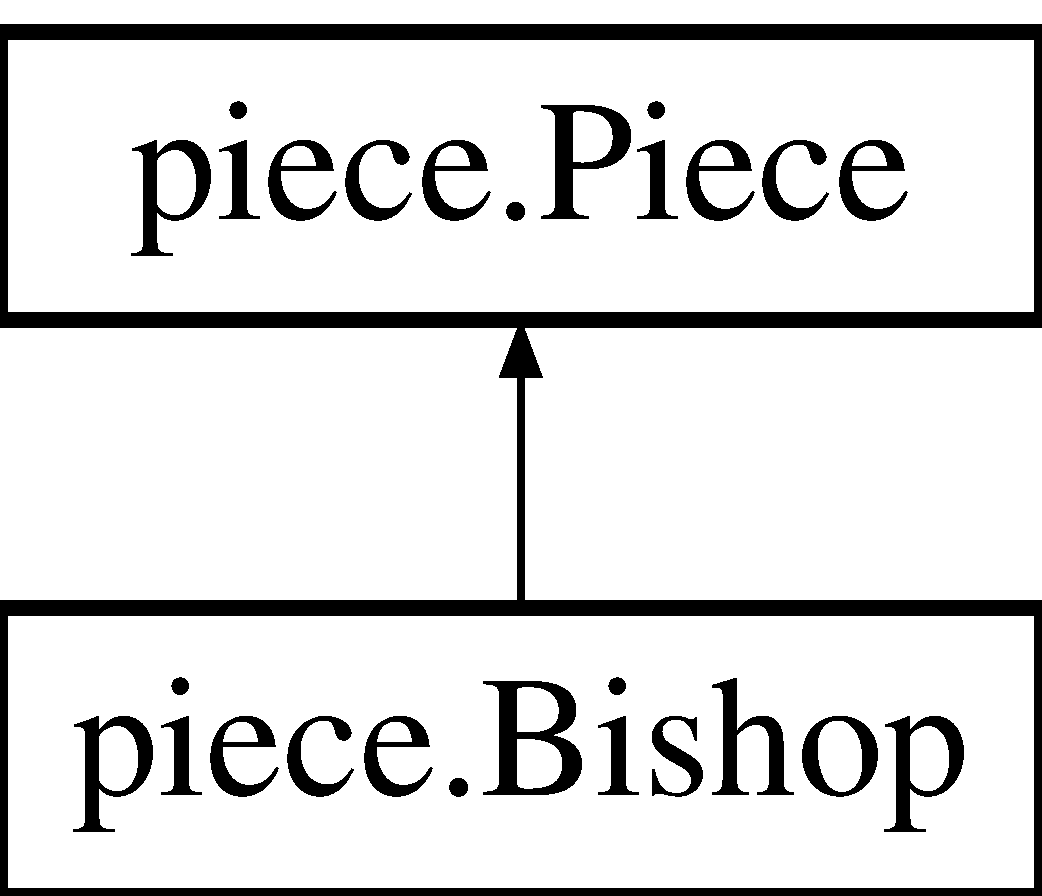
\includegraphics[height=2.000000cm]{classpiece_1_1Bishop}
\end{center}
\end{figure}
\subsection*{Public Member Functions}
\begin{DoxyCompactItemize}
\item 
void \hyperlink{classpiece_1_1Bishop_af3af2a374601e579cd5249b7951f0c81}{update\-Moves} (\hyperlink{classmodel_1_1Board}{Board} board)
\end{DoxyCompactItemize}
\subsection*{Additional Inherited Members}


\subsection{Member Function Documentation}
\hypertarget{classpiece_1_1Bishop_af3af2a374601e579cd5249b7951f0c81}{\index{piece\-::\-Bishop@{piece\-::\-Bishop}!update\-Moves@{update\-Moves}}
\index{update\-Moves@{update\-Moves}!piece::Bishop@{piece\-::\-Bishop}}
\subsubsection[{update\-Moves}]{\setlength{\rightskip}{0pt plus 5cm}void piece.\-Bishop.\-update\-Moves (
\begin{DoxyParamCaption}
\item[{{\bf Board}}]{board}
\end{DoxyParamCaption}
)\hspace{0.3cm}{\ttfamily [inline]}, {\ttfamily [virtual]}}}\label{classpiece_1_1Bishop_af3af2a374601e579cd5249b7951f0c81}
Upates the possible moves for a given piece. 
\begin{DoxyParams}{Parameters}
{\em spaces} & The state of the chess board. \\
\hline
\end{DoxyParams}


Implements \hyperlink{classpiece_1_1Piece_a4dbb3f3506bfc5c4a2015182857d08e0}{piece.\-Piece}.



The documentation for this class was generated from the following file\-:\begin{DoxyCompactItemize}
\item 
piece/Bishop.\-java\end{DoxyCompactItemize}

\hypertarget{classtest_1_1BishopTest}{\section{test.\-Bishop\-Test Class Reference}
\label{classtest_1_1BishopTest}\index{test.\-Bishop\-Test@{test.\-Bishop\-Test}}
}
\subsection*{Public Member Functions}
\begin{DoxyCompactItemize}
\item 
\hypertarget{classtest_1_1BishopTest_a58b9802c94c002fd4bb4ac676fd17fda}{void {\bfseries set\-Up} ()  throws Exception }\label{classtest_1_1BishopTest_a58b9802c94c002fd4bb4ac676fd17fda}

\item 
\hypertarget{classtest_1_1BishopTest_a907048258e752fe2419ba11ae7cea221}{void {\bfseries bishop\-Move} ()}\label{classtest_1_1BishopTest_a907048258e752fe2419ba11ae7cea221}

\item 
\hypertarget{classtest_1_1BishopTest_a39b6d5b8258787d4c68c7a88214fc30d}{void {\bfseries illegal\-Move} ()}\label{classtest_1_1BishopTest_a39b6d5b8258787d4c68c7a88214fc30d}

\item 
\hypertarget{classtest_1_1BishopTest_afcc606196bd42595b31a6f3bdf552998}{void {\bfseries capture\-Own\-Pieces} ()}\label{classtest_1_1BishopTest_afcc606196bd42595b31a6f3bdf552998}

\item 
\hypertarget{classtest_1_1BishopTest_aac4d4da8ff982822f541508b8fb970b0}{void {\bfseries jump\-Own\-Pieces} ()}\label{classtest_1_1BishopTest_aac4d4da8ff982822f541508b8fb970b0}

\item 
\hypertarget{classtest_1_1BishopTest_a4c9f847b1ef661b2e099dada3c7b3741}{void {\bfseries capture\-Enemy} ()}\label{classtest_1_1BishopTest_a4c9f847b1ef661b2e099dada3c7b3741}

\item 
\hypertarget{classtest_1_1BishopTest_a635a251082b8150fb91b6eb389965af2}{void {\bfseries jump\-Enemy\-Pieces} ()}\label{classtest_1_1BishopTest_a635a251082b8150fb91b6eb389965af2}

\end{DoxyCompactItemize}


The documentation for this class was generated from the following file\-:\begin{DoxyCompactItemize}
\item 
test/Bishop\-Test.\-java\end{DoxyCompactItemize}

\hypertarget{classmodel_1_1Board}{\section{model.\-Board Class Reference}
\label{classmodel_1_1Board}\index{model.\-Board@{model.\-Board}}
}
\subsection*{Public Member Functions}
\begin{DoxyCompactItemize}
\item 
\hyperlink{classmodel_1_1Board_aac7c0f18953f62b56fe1631dedc218ea}{Board} (\hyperlink{classmodel_1_1Board}{Board} other)
\item 
void \hyperlink{classmodel_1_1Board_ac230b4f661035db4d987134a91ab5cd4}{copy} (\hyperlink{classmodel_1_1Board}{Board} other)
\item 
\hypertarget{classmodel_1_1Board_a63d8dd9b3dc145e23e0d41295db354f3}{Piece\mbox{[}$\,$\mbox{]}\mbox{[}$\,$\mbox{]} {\bfseries get\-Spaces} ()}\label{classmodel_1_1Board_a63d8dd9b3dc145e23e0d41295db354f3}

\item 
\hypertarget{classmodel_1_1Board_a13f1f3a8a516e662029745977b45225d}{void {\bfseries set\-Spaces} (Piece\mbox{[}$\,$\mbox{]}\mbox{[}$\,$\mbox{]} spaces)}\label{classmodel_1_1Board_a13f1f3a8a516e662029745977b45225d}

\item 
void \hyperlink{classmodel_1_1Board_ab04268464780a556231843bfaca1f7bc}{reset} ()
\end{DoxyCompactItemize}
\subsection*{Public Attributes}
\begin{DoxyCompactItemize}
\item 
\hypertarget{classmodel_1_1Board_a2f1a9f701bbe38b93555d41ce47eef47}{Piece\mbox{[}$\,$\mbox{]}\mbox{[}$\,$\mbox{]} {\bfseries spaces} = null}\label{classmodel_1_1Board_a2f1a9f701bbe38b93555d41ce47eef47}

\end{DoxyCompactItemize}


\subsection{Detailed Description}
\begin{DoxyAuthor}{Author}
Will 
\end{DoxyAuthor}


\subsection{Constructor \& Destructor Documentation}
\hypertarget{classmodel_1_1Board_aac7c0f18953f62b56fe1631dedc218ea}{\index{model\-::\-Board@{model\-::\-Board}!Board@{Board}}
\index{Board@{Board}!model::Board@{model\-::\-Board}}
\subsubsection[{Board}]{\setlength{\rightskip}{0pt plus 5cm}model.\-Board.\-Board (
\begin{DoxyParamCaption}
\item[{{\bf Board}}]{other}
\end{DoxyParamCaption}
)\hspace{0.3cm}{\ttfamily [inline]}}}\label{classmodel_1_1Board_aac7c0f18953f62b56fe1631dedc218ea}
Copy constructor 
\begin{DoxyParams}{Parameters}
{\em other} & the board to copy \\
\hline
\end{DoxyParams}


\subsection{Member Function Documentation}
\hypertarget{classmodel_1_1Board_ac230b4f661035db4d987134a91ab5cd4}{\index{model\-::\-Board@{model\-::\-Board}!copy@{copy}}
\index{copy@{copy}!model::Board@{model\-::\-Board}}
\subsubsection[{copy}]{\setlength{\rightskip}{0pt plus 5cm}void model.\-Board.\-copy (
\begin{DoxyParamCaption}
\item[{{\bf Board}}]{other}
\end{DoxyParamCaption}
)\hspace{0.3cm}{\ttfamily [inline]}}}\label{classmodel_1_1Board_ac230b4f661035db4d987134a91ab5cd4}
A copy helper function that performs a deep copy of every element in the other board. 
\begin{DoxyParams}{Parameters}
{\em other} & \\
\hline
\end{DoxyParams}
\hypertarget{classmodel_1_1Board_ab04268464780a556231843bfaca1f7bc}{\index{model\-::\-Board@{model\-::\-Board}!reset@{reset}}
\index{reset@{reset}!model::Board@{model\-::\-Board}}
\subsubsection[{reset}]{\setlength{\rightskip}{0pt plus 5cm}void model.\-Board.\-reset (
\begin{DoxyParamCaption}
{}
\end{DoxyParamCaption}
)\hspace{0.3cm}{\ttfamily [inline]}}}\label{classmodel_1_1Board_ab04268464780a556231843bfaca1f7bc}
Restarts the current board to the unitialized state with no pieces. 

The documentation for this class was generated from the following file\-:\begin{DoxyCompactItemize}
\item 
model/Board.\-java\end{DoxyCompactItemize}

\hypertarget{classlogic_1_1BoardLogic}{\section{logic.\-Board\-Logic Class Reference}
\label{classlogic_1_1BoardLogic}\index{logic.\-Board\-Logic@{logic.\-Board\-Logic}}
}
\subsection*{Static Public Member Functions}
\begin{DoxyCompactItemize}
\item 
static void \hyperlink{classlogic_1_1BoardLogic_a8805b83ab700a29dcc71d66803199adf}{update\-Pieces} (\hyperlink{classmodel_1_1Board}{Board} board)
\item 
static boolean \hyperlink{classlogic_1_1BoardLogic_a1117819fcc1471cb01799198d14f3e4c}{in\-Check} (\hyperlink{classmodel_1_1Board}{Board} board, Color player)
\item 
static boolean \hyperlink{classlogic_1_1BoardLogic_ab5d863552542c372796ceff388e6a42b}{in\-Checkmate} (\hyperlink{classmodel_1_1Board}{Board} board, Color player)
\item 
static boolean \hyperlink{classlogic_1_1BoardLogic_accfe2bf1822c3b6abbcb66cb2e78e7b9}{in\-Stalemate} (\hyperlink{classmodel_1_1Board}{Board} board, Color player)
\item 
static Vector$<$ \hyperlink{classmodel_1_1Space}{Space} $>$ \hyperlink{classlogic_1_1BoardLogic_a1362b857bf585f1bfe2a1b55377d3ae6}{moves\-On\-Board} (\hyperlink{classmodel_1_1Board}{Board} board, \hyperlink{classpiece_1_1Piece}{Piece} piece)
\item 
static boolean \hyperlink{classlogic_1_1BoardLogic_a20d53bc0146f9c90598880bd8f731fe4}{move\-Piece} (\hyperlink{classmodel_1_1Board}{Board} board, \hyperlink{classpiece_1_1Piece}{Piece} piece, int rtarget, int ftarget)
\item 
static boolean \hyperlink{classlogic_1_1BoardLogic_a5fec15d32e299f21a067c90a1d28afbf}{set\-Piece} (\hyperlink{classmodel_1_1Board}{Board} board, \hyperlink{classpiece_1_1Piece}{Piece} piece, int rank, int file, Color player)
\item 
static \hyperlink{classpiece_1_1Piece}{Piece} \hyperlink{classlogic_1_1BoardLogic_ad087d5f282d8bc4291263a2135dd3466}{get\-Piece} (\hyperlink{classmodel_1_1Board}{Board} board, int rank, int file)
\item 
static boolean \hyperlink{classlogic_1_1BoardLogic_a84fa3af836d6218a29167e97f22962fe}{out\-Of\-Bounds} (\hyperlink{classmodel_1_1Board}{Board} board, int rank, int file)
\end{DoxyCompactItemize}


\subsection{Member Function Documentation}
\hypertarget{classlogic_1_1BoardLogic_ad087d5f282d8bc4291263a2135dd3466}{\index{logic\-::\-Board\-Logic@{logic\-::\-Board\-Logic}!get\-Piece@{get\-Piece}}
\index{get\-Piece@{get\-Piece}!logic::BoardLogic@{logic\-::\-Board\-Logic}}
\subsubsection[{get\-Piece}]{\setlength{\rightskip}{0pt plus 5cm}static {\bf Piece} logic.\-Board\-Logic.\-get\-Piece (
\begin{DoxyParamCaption}
\item[{{\bf Board}}]{board, }
\item[{int}]{rank, }
\item[{int}]{file}
\end{DoxyParamCaption}
)\hspace{0.3cm}{\ttfamily [inline]}, {\ttfamily [static]}}}\label{classlogic_1_1BoardLogic_ad087d5f282d8bc4291263a2135dd3466}
Get piece on board 
\begin{DoxyParams}{Parameters}
{\em board} & the board to get piece \\
\hline
{\em rank} & the x (rank) location of the piece \\
\hline
{\em file} & the y (file) location of the piece \\
\hline
\end{DoxyParams}
\begin{DoxyReturn}{Returns}
the piece at a given space 
\end{DoxyReturn}
\hypertarget{classlogic_1_1BoardLogic_a1117819fcc1471cb01799198d14f3e4c}{\index{logic\-::\-Board\-Logic@{logic\-::\-Board\-Logic}!in\-Check@{in\-Check}}
\index{in\-Check@{in\-Check}!logic::BoardLogic@{logic\-::\-Board\-Logic}}
\subsubsection[{in\-Check}]{\setlength{\rightskip}{0pt plus 5cm}static boolean logic.\-Board\-Logic.\-in\-Check (
\begin{DoxyParamCaption}
\item[{{\bf Board}}]{board, }
\item[{Color}]{player}
\end{DoxyParamCaption}
)\hspace{0.3cm}{\ttfamily [inline]}, {\ttfamily [static]}}}\label{classlogic_1_1BoardLogic_a1117819fcc1471cb01799198d14f3e4c}

\begin{DoxyParams}{Parameters}
{\em board} & the board to check whether the player is in\-Check \\
\hline
{\em player} & the color of the player check for check \\
\hline
\end{DoxyParams}
\begin{DoxyReturn}{Returns}
true if the given player is in check 
\end{DoxyReturn}
\hypertarget{classlogic_1_1BoardLogic_ab5d863552542c372796ceff388e6a42b}{\index{logic\-::\-Board\-Logic@{logic\-::\-Board\-Logic}!in\-Checkmate@{in\-Checkmate}}
\index{in\-Checkmate@{in\-Checkmate}!logic::BoardLogic@{logic\-::\-Board\-Logic}}
\subsubsection[{in\-Checkmate}]{\setlength{\rightskip}{0pt plus 5cm}static boolean logic.\-Board\-Logic.\-in\-Checkmate (
\begin{DoxyParamCaption}
\item[{{\bf Board}}]{board, }
\item[{Color}]{player}
\end{DoxyParamCaption}
)\hspace{0.3cm}{\ttfamily [inline]}, {\ttfamily [static]}}}\label{classlogic_1_1BoardLogic_ab5d863552542c372796ceff388e6a42b}

\begin{DoxyParams}{Parameters}
{\em board} & the board to to check whether the player is in\-Checkmate \\
\hline
{\em player} & the color of the player to check for checkmate \\
\hline
\end{DoxyParams}
\begin{DoxyReturn}{Returns}
true if the given player is in checkmate 
\end{DoxyReturn}
\hypertarget{classlogic_1_1BoardLogic_accfe2bf1822c3b6abbcb66cb2e78e7b9}{\index{logic\-::\-Board\-Logic@{logic\-::\-Board\-Logic}!in\-Stalemate@{in\-Stalemate}}
\index{in\-Stalemate@{in\-Stalemate}!logic::BoardLogic@{logic\-::\-Board\-Logic}}
\subsubsection[{in\-Stalemate}]{\setlength{\rightskip}{0pt plus 5cm}static boolean logic.\-Board\-Logic.\-in\-Stalemate (
\begin{DoxyParamCaption}
\item[{{\bf Board}}]{board, }
\item[{Color}]{player}
\end{DoxyParamCaption}
)\hspace{0.3cm}{\ttfamily [inline]}, {\ttfamily [static]}}}\label{classlogic_1_1BoardLogic_accfe2bf1822c3b6abbcb66cb2e78e7b9}

\begin{DoxyParams}{Parameters}
{\em board} & the board to check whether the player is in\-Stalemate \\
\hline
{\em player} & the color of player to check for stalemate \\
\hline
\end{DoxyParams}
\begin{DoxyReturn}{Returns}
true if in stalemate 
\end{DoxyReturn}
\hypertarget{classlogic_1_1BoardLogic_a20d53bc0146f9c90598880bd8f731fe4}{\index{logic\-::\-Board\-Logic@{logic\-::\-Board\-Logic}!move\-Piece@{move\-Piece}}
\index{move\-Piece@{move\-Piece}!logic::BoardLogic@{logic\-::\-Board\-Logic}}
\subsubsection[{move\-Piece}]{\setlength{\rightskip}{0pt plus 5cm}static boolean logic.\-Board\-Logic.\-move\-Piece (
\begin{DoxyParamCaption}
\item[{{\bf Board}}]{board, }
\item[{{\bf Piece}}]{piece, }
\item[{int}]{rtarget, }
\item[{int}]{ftarget}
\end{DoxyParamCaption}
)\hspace{0.3cm}{\ttfamily [inline]}, {\ttfamily [static]}}}\label{classlogic_1_1BoardLogic_a20d53bc0146f9c90598880bd8f731fe4}
Moves a piece on the board from (rstart,fstart) to (rtarget,ftarget). 
\begin{DoxyParams}{Parameters}
{\em board} & the board to move piece \\
\hline
{\em piece} & the piece to be moved \\
\hline
{\em rtarget} & the target rank (x position) of the move \\
\hline
{\em ftarget} & the target file (y position) of the move \\
\hline
\end{DoxyParams}
\begin{DoxyReturn}{Returns}
1 if out\-Of\-Bound, 2 if it's the same owner, false otherwise 
\end{DoxyReturn}
\hypertarget{classlogic_1_1BoardLogic_a1362b857bf585f1bfe2a1b55377d3ae6}{\index{logic\-::\-Board\-Logic@{logic\-::\-Board\-Logic}!moves\-On\-Board@{moves\-On\-Board}}
\index{moves\-On\-Board@{moves\-On\-Board}!logic::BoardLogic@{logic\-::\-Board\-Logic}}
\subsubsection[{moves\-On\-Board}]{\setlength{\rightskip}{0pt plus 5cm}static Vector$<${\bf Space}$>$ logic.\-Board\-Logic.\-moves\-On\-Board (
\begin{DoxyParamCaption}
\item[{{\bf Board}}]{board, }
\item[{{\bf Piece}}]{piece}
\end{DoxyParamCaption}
)\hspace{0.3cm}{\ttfamily [inline]}, {\ttfamily [static]}}}\label{classlogic_1_1BoardLogic_a1362b857bf585f1bfe2a1b55377d3ae6}

\begin{DoxyParams}{Parameters}
{\em board} & \\
\hline
{\em piece} & \\
\hline
\end{DoxyParams}
\begin{DoxyReturn}{Returns}
available moves of piece on board 
\end{DoxyReturn}
\hypertarget{classlogic_1_1BoardLogic_a84fa3af836d6218a29167e97f22962fe}{\index{logic\-::\-Board\-Logic@{logic\-::\-Board\-Logic}!out\-Of\-Bounds@{out\-Of\-Bounds}}
\index{out\-Of\-Bounds@{out\-Of\-Bounds}!logic::BoardLogic@{logic\-::\-Board\-Logic}}
\subsubsection[{out\-Of\-Bounds}]{\setlength{\rightskip}{0pt plus 5cm}static boolean logic.\-Board\-Logic.\-out\-Of\-Bounds (
\begin{DoxyParamCaption}
\item[{{\bf Board}}]{board, }
\item[{int}]{rank, }
\item[{int}]{file}
\end{DoxyParamCaption}
)\hspace{0.3cm}{\ttfamily [inline]}, {\ttfamily [static]}}}\label{classlogic_1_1BoardLogic_a84fa3af836d6218a29167e97f22962fe}
Helper function that checks whether a given (rank,file) pair is within the board range. 
\begin{DoxyParams}{Parameters}
{\em board} & the board to check \\
\hline
{\em rank} & the x (rank) location of the piece \\
\hline
{\em file} & the y (file) location of the piece \\
\hline
\end{DoxyParams}
\begin{DoxyReturn}{Returns}
true if the position given is not a valid board position. 
\end{DoxyReturn}
\hypertarget{classlogic_1_1BoardLogic_a5fec15d32e299f21a067c90a1d28afbf}{\index{logic\-::\-Board\-Logic@{logic\-::\-Board\-Logic}!set\-Piece@{set\-Piece}}
\index{set\-Piece@{set\-Piece}!logic::BoardLogic@{logic\-::\-Board\-Logic}}
\subsubsection[{set\-Piece}]{\setlength{\rightskip}{0pt plus 5cm}static boolean logic.\-Board\-Logic.\-set\-Piece (
\begin{DoxyParamCaption}
\item[{{\bf Board}}]{board, }
\item[{{\bf Piece}}]{piece, }
\item[{int}]{rank, }
\item[{int}]{file, }
\item[{Color}]{player}
\end{DoxyParamCaption}
)\hspace{0.3cm}{\ttfamily [inline]}, {\ttfamily [static]}}}\label{classlogic_1_1BoardLogic_a5fec15d32e299f21a067c90a1d28afbf}
Set piece on board 
\begin{DoxyParams}{Parameters}
{\em board} & the board to set piece \\
\hline
{\em piece} & the piece to set \\
\hline
{\em rank} & the x (rank) location of the piece \\
\hline
{\em file} & the y (file) location of the piece \\
\hline
{\em player} & the owner of the piece (W\-H\-I\-T\-E,B\-L\-A\-C\-K) \\
\hline
\end{DoxyParams}
\begin{DoxyReturn}{Returns}
true if the piece was set successfully 
\end{DoxyReturn}
\hypertarget{classlogic_1_1BoardLogic_a8805b83ab700a29dcc71d66803199adf}{\index{logic\-::\-Board\-Logic@{logic\-::\-Board\-Logic}!update\-Pieces@{update\-Pieces}}
\index{update\-Pieces@{update\-Pieces}!logic::BoardLogic@{logic\-::\-Board\-Logic}}
\subsubsection[{update\-Pieces}]{\setlength{\rightskip}{0pt plus 5cm}static void logic.\-Board\-Logic.\-update\-Pieces (
\begin{DoxyParamCaption}
\item[{{\bf Board}}]{board}
\end{DoxyParamCaption}
)\hspace{0.3cm}{\ttfamily [inline]}, {\ttfamily [static]}}}\label{classlogic_1_1BoardLogic_a8805b83ab700a29dcc71d66803199adf}
We need to maintain possible moves for each piece to detect game-\/ending conditions. 
\begin{DoxyParams}{Parameters}
{\em board} & the board to update pieces \\
\hline
\end{DoxyParams}


The documentation for this class was generated from the following file\-:\begin{DoxyCompactItemize}
\item 
logic/Board\-Logic.\-java\end{DoxyCompactItemize}

\hypertarget{classtest_1_1BoardTest}{\section{test.\-Board\-Test Class Reference}
\label{classtest_1_1BoardTest}\index{test.\-Board\-Test@{test.\-Board\-Test}}
}
\subsection*{Public Member Functions}
\begin{DoxyCompactItemize}
\item 
\hypertarget{classtest_1_1BoardTest_ae6d37c5be726446c186c70b1efc00916}{void {\bfseries set\-Up} ()}\label{classtest_1_1BoardTest_ae6d37c5be726446c186c70b1efc00916}

\item 
\hypertarget{classtest_1_1BoardTest_a3ec0792fa88545e83de0f9319875a378}{void {\bfseries empty\-Constructor} ()}\label{classtest_1_1BoardTest_a3ec0792fa88545e83de0f9319875a378}

\item 
\hypertarget{classtest_1_1BoardTest_afc3c18de1c56b9f37fce53519933eaeb}{void {\bfseries not\-In\-Check} ()}\label{classtest_1_1BoardTest_afc3c18de1c56b9f37fce53519933eaeb}

\item 
\hypertarget{classtest_1_1BoardTest_a735d51ed62a3173efdee865248a5767c}{void {\bfseries not\-In\-Own\-Check} ()}\label{classtest_1_1BoardTest_a735d51ed62a3173efdee865248a5767c}

\item 
\hypertarget{classtest_1_1BoardTest_a895ee333ab28bf431c0b4d31924cc274}{void {\bfseries opponent\-In\-Check} ()}\label{classtest_1_1BoardTest_a895ee333ab28bf431c0b4d31924cc274}

\item 
\hypertarget{classtest_1_1BoardTest_adb9fdfc2c872dbdad738bead1e79c03e}{void {\bfseries move\-Into\-Check} ()}\label{classtest_1_1BoardTest_adb9fdfc2c872dbdad738bead1e79c03e}

\item 
\hypertarget{classtest_1_1BoardTest_a8e0afe9c075e09d51cc21405a932417c}{void {\bfseries move\-Other\-Piece\-In\-Check} ()}\label{classtest_1_1BoardTest_a8e0afe9c075e09d51cc21405a932417c}

\item 
\hypertarget{classtest_1_1BoardTest_ada6bc8c11890b19b6a9386d180304d85}{void {\bfseries capture\-Outof\-Check} ()}\label{classtest_1_1BoardTest_ada6bc8c11890b19b6a9386d180304d85}

\item 
\hypertarget{classtest_1_1BoardTest_aac0671a1d28175f82fe7ebd8a7834ec2}{void {\bfseries capture\-Into\-Check} ()}\label{classtest_1_1BoardTest_aac0671a1d28175f82fe7ebd8a7834ec2}

\item 
\hypertarget{classtest_1_1BoardTest_ab854addb0a5a79e2a1521f0b4e39ac0c}{void {\bfseries empty\-Board\-Check} ()}\label{classtest_1_1BoardTest_ab854addb0a5a79e2a1521f0b4e39ac0c}

\item 
\hypertarget{classtest_1_1BoardTest_a2de7c677b39c58e7670b959688da9e3b}{void {\bfseries not\-In\-Friendly\-Checkmate} ()}\label{classtest_1_1BoardTest_a2de7c677b39c58e7670b959688da9e3b}

\item 
\hypertarget{classtest_1_1BoardTest_a2cdf01a22f538f77cd4b9cfa43e4afa6}{void {\bfseries opponent\-In\-Checkmate} ()}\label{classtest_1_1BoardTest_a2cdf01a22f538f77cd4b9cfa43e4afa6}

\item 
\hypertarget{classtest_1_1BoardTest_a484ad2fd7123bdf6a35b9bd63821a13d}{void {\bfseries not\-In\-Check\-Or\-Check\-Mate} ()}\label{classtest_1_1BoardTest_a484ad2fd7123bdf6a35b9bd63821a13d}

\item 
\hypertarget{classtest_1_1BoardTest_aaab5644302b3794b87cf897f21fd1915}{void {\bfseries not\-In\-Check\-Mate} ()}\label{classtest_1_1BoardTest_aaab5644302b3794b87cf897f21fd1915}

\item 
\hypertarget{classtest_1_1BoardTest_acd4d2afb62f5255537b55a0ec2f8eb5d}{void {\bfseries empyt\-Board\-Check\-Mate} ()}\label{classtest_1_1BoardTest_acd4d2afb62f5255537b55a0ec2f8eb5d}

\item 
\hypertarget{classtest_1_1BoardTest_ab0f9ff6f618d19a64153d0096392eaef}{void {\bfseries in\-Stalemate} ()}\label{classtest_1_1BoardTest_ab0f9ff6f618d19a64153d0096392eaef}

\item 
\hypertarget{classtest_1_1BoardTest_af6aa06646303d5a37ec42d2c42e98a60}{void {\bfseries empty\-Board\-Stalemate} ()}\label{classtest_1_1BoardTest_af6aa06646303d5a37ec42d2c42e98a60}

\item 
\hypertarget{classtest_1_1BoardTest_a772af9b2ab858b438ae74e09a0ca7c19}{void {\bfseries no\-Stalemate\-In\-Check} ()}\label{classtest_1_1BoardTest_a772af9b2ab858b438ae74e09a0ca7c19}

\item 
\hypertarget{classtest_1_1BoardTest_af4b03eee98fdbf834d2624292bc0b6bf}{void {\bfseries no\-Check\-No\-Stalemate} ()}\label{classtest_1_1BoardTest_af4b03eee98fdbf834d2624292bc0b6bf}

\end{DoxyCompactItemize}


The documentation for this class was generated from the following file\-:\begin{DoxyCompactItemize}
\item 
test/Board\-Test.\-java\end{DoxyCompactItemize}

\hypertarget{classview_1_1ChessGui_1_1BoardWindow}{\section{view.\-Chess\-Gui.\-Board\-Window Class Reference}
\label{classview_1_1ChessGui_1_1BoardWindow}\index{view.\-Chess\-Gui.\-Board\-Window@{view.\-Chess\-Gui.\-Board\-Window}}
}
Inheritance diagram for view.\-Chess\-Gui.\-Board\-Window\-:\begin{figure}[H]
\begin{center}
\leavevmode
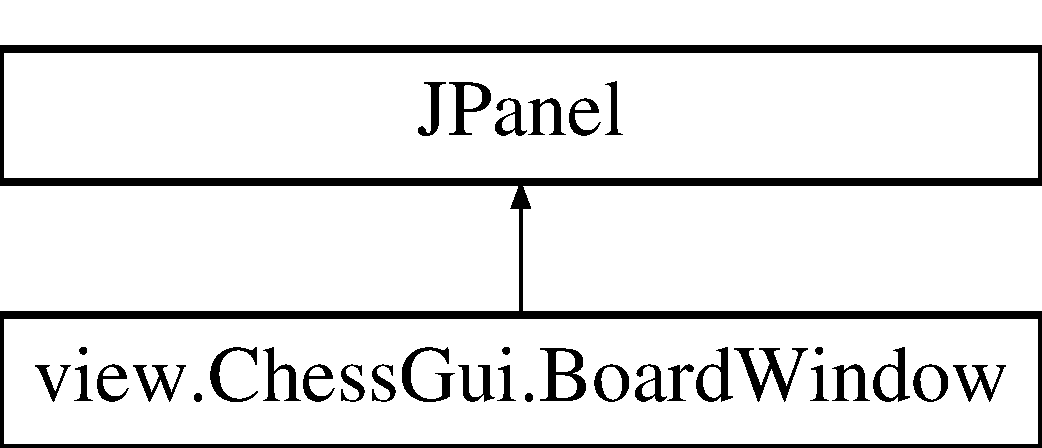
\includegraphics[height=2.000000cm]{classview_1_1ChessGui_1_1BoardWindow}
\end{center}
\end{figure}


The documentation for this class was generated from the following file\-:\begin{DoxyCompactItemize}
\item 
view/Chess\-Gui.\-java\end{DoxyCompactItemize}

\hypertarget{classview_1_1ChessGui}{\section{view.\-Chess\-Gui Class Reference}
\label{classview_1_1ChessGui}\index{view.\-Chess\-Gui@{view.\-Chess\-Gui}}
}
Inheritance diagram for view.\-Chess\-Gui\-:\begin{figure}[H]
\begin{center}
\leavevmode
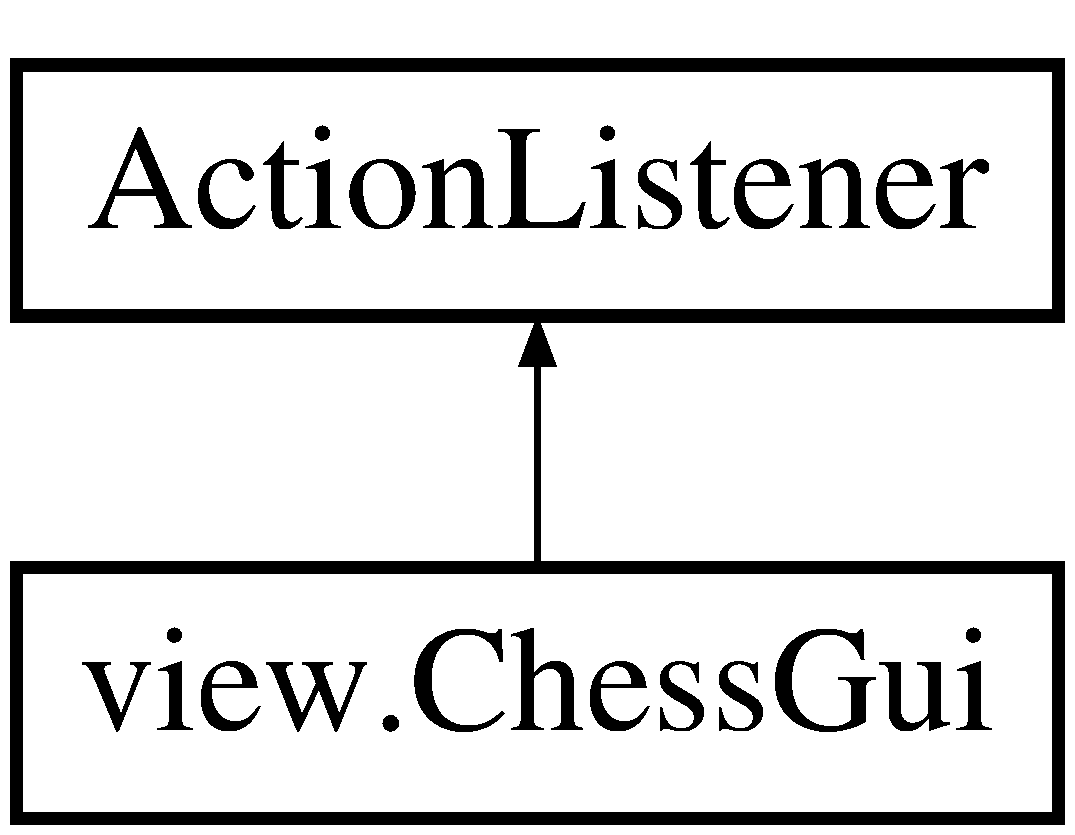
\includegraphics[height=2.000000cm]{classview_1_1ChessGui}
\end{center}
\end{figure}
\subsection*{Classes}
\begin{DoxyCompactItemize}
\item 
class \hyperlink{classview_1_1ChessGui_1_1BoardWindow}{Board\-Window}
\item 
class {\bfseries My\-Action\-Listener}
\end{DoxyCompactItemize}
\subsection*{Public Member Functions}
\begin{DoxyCompactItemize}
\item 
\hypertarget{classview_1_1ChessGui_aa50c2d1a70a911eb1eb34edd39248d0f}{void {\bfseries action\-Performed} (Action\-Event e)}\label{classview_1_1ChessGui_aa50c2d1a70a911eb1eb34edd39248d0f}

\end{DoxyCompactItemize}
\subsection*{Static Public Member Functions}
\begin{DoxyCompactItemize}
\item 
\hypertarget{classview_1_1ChessGui_a8043eb548c095e1455b38c499d221458}{static void {\bfseries main} (String\mbox{[}$\,$\mbox{]} args)}\label{classview_1_1ChessGui_a8043eb548c095e1455b38c499d221458}

\end{DoxyCompactItemize}


The documentation for this class was generated from the following file\-:\begin{DoxyCompactItemize}
\item 
view/Chess\-Gui.\-java\end{DoxyCompactItemize}

\hypertarget{classcontroller_1_1Game}{\section{controller.\-Game Class Reference}
\label{classcontroller_1_1Game}\index{controller.\-Game@{controller.\-Game}}
}
\subsection*{Public Member Functions}
\begin{DoxyCompactItemize}
\item 
\hypertarget{classcontroller_1_1Game_ab16ee51cf48633d3d072a964de234b2b}{void {\bfseries set\-Board} ()}\label{classcontroller_1_1Game_ab16ee51cf48633d3d072a964de234b2b}

\item 
\hypertarget{classcontroller_1_1Game_af83607dbad5e6502359af3d97b05da3b}{void {\bfseries set\-Players} (String player1, String player2)}\label{classcontroller_1_1Game_af83607dbad5e6502359af3d97b05da3b}

\item 
\hypertarget{classcontroller_1_1Game_a5bee55ed8349d171a0d2cbdf4aa767d4}{\hyperlink{classcontroller_1_1Player}{Player} {\bfseries next\-Player} (\hyperlink{classcontroller_1_1Player}{Player} curr\-Player)}\label{classcontroller_1_1Game_a5bee55ed8349d171a0d2cbdf4aa767d4}

\item 
\hypertarget{classcontroller_1_1Game_abb852409646b9ea9a1565eb875d7d3ca}{void {\bfseries restart} (\hyperlink{classcontroller_1_1Player}{Player} curr\-Player)}\label{classcontroller_1_1Game_abb852409646b9ea9a1565eb875d7d3ca}

\end{DoxyCompactItemize}
\subsection*{Public Attributes}
\begin{DoxyCompactItemize}
\item 
\hypertarget{classcontroller_1_1Game_ad5a94f775d7191c1b0f77cc905a5a643}{Board {\bfseries game\-Board}}\label{classcontroller_1_1Game_ad5a94f775d7191c1b0f77cc905a5a643}

\item 
\hypertarget{classcontroller_1_1Game_a8e286412b3a4268a729727d6ed906a58}{\hyperlink{classcontroller_1_1Player}{Player} {\bfseries player1}}\label{classcontroller_1_1Game_a8e286412b3a4268a729727d6ed906a58}

\item 
\hypertarget{classcontroller_1_1Game_a5b5a4b59882c8d5f921daa1cc2a53b5a}{Stack$<$ \hyperlink{classcontroller_1_1Step}{Step} $>$ {\bfseries move} = new Stack$<$\hyperlink{classcontroller_1_1Step}{Step}$>$()}\label{classcontroller_1_1Game_a5b5a4b59882c8d5f921daa1cc2a53b5a}

\end{DoxyCompactItemize}


The documentation for this class was generated from the following file\-:\begin{DoxyCompactItemize}
\item 
controller/Game.\-java\end{DoxyCompactItemize}

\hypertarget{classview_1_1GameLoop}{\section{view.\-Game\-Loop Class Reference}
\label{classview_1_1GameLoop}\index{view.\-Game\-Loop@{view.\-Game\-Loop}}
}


The documentation for this class was generated from the following file\-:\begin{DoxyCompactItemize}
\item 
view/Game\-Loop.\-java\end{DoxyCompactItemize}

\hypertarget{classpiece_1_1King}{\section{piece.\-King Class Reference}
\label{classpiece_1_1King}\index{piece.\-King@{piece.\-King}}
}
Inheritance diagram for piece.\-King\-:\begin{figure}[H]
\begin{center}
\leavevmode
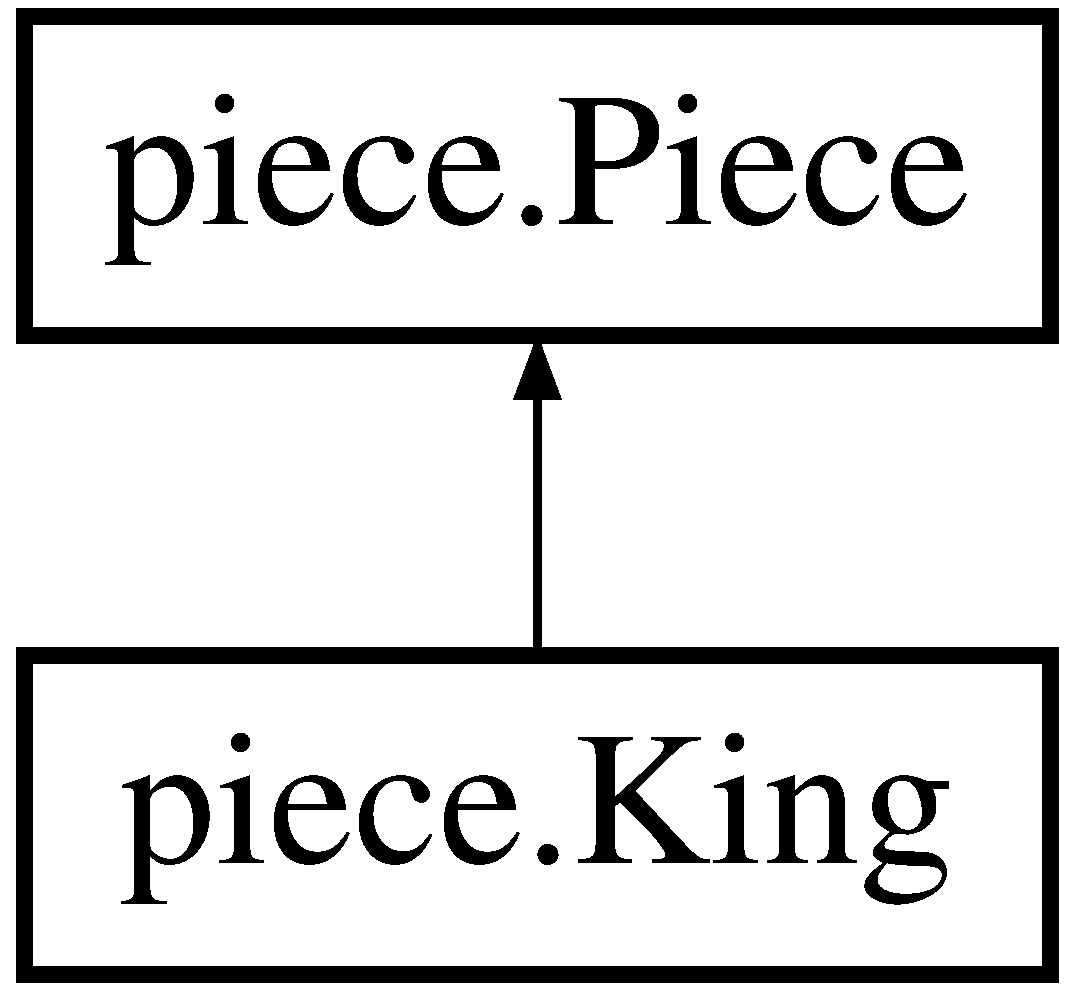
\includegraphics[height=2.000000cm]{classpiece_1_1King}
\end{center}
\end{figure}
\subsection*{Public Member Functions}
\begin{DoxyCompactItemize}
\item 
void \hyperlink{classpiece_1_1King_a93304e2c4a5b94acc2c4606a9d2a9f4e}{update\-Moves} (\hyperlink{classmodel_1_1Board}{Board} board)
\end{DoxyCompactItemize}
\subsection*{Additional Inherited Members}


\subsection{Member Function Documentation}
\hypertarget{classpiece_1_1King_a93304e2c4a5b94acc2c4606a9d2a9f4e}{\index{piece\-::\-King@{piece\-::\-King}!update\-Moves@{update\-Moves}}
\index{update\-Moves@{update\-Moves}!piece::King@{piece\-::\-King}}
\subsubsection[{update\-Moves}]{\setlength{\rightskip}{0pt plus 5cm}void piece.\-King.\-update\-Moves (
\begin{DoxyParamCaption}
\item[{{\bf Board}}]{board}
\end{DoxyParamCaption}
)\hspace{0.3cm}{\ttfamily [inline]}, {\ttfamily [virtual]}}}\label{classpiece_1_1King_a93304e2c4a5b94acc2c4606a9d2a9f4e}
Upates the possible moves for a given piece. 
\begin{DoxyParams}{Parameters}
{\em spaces} & The state of the chess board. \\
\hline
\end{DoxyParams}


Implements \hyperlink{classpiece_1_1Piece_a4dbb3f3506bfc5c4a2015182857d08e0}{piece.\-Piece}.



The documentation for this class was generated from the following file\-:\begin{DoxyCompactItemize}
\item 
piece/King.\-java\end{DoxyCompactItemize}

\hypertarget{classtest_1_1KingTest}{\section{test.\-King\-Test Class Reference}
\label{classtest_1_1KingTest}\index{test.\-King\-Test@{test.\-King\-Test}}
}
\subsection*{Public Member Functions}
\begin{DoxyCompactItemize}
\item 
\hypertarget{classtest_1_1KingTest_a1da7d245e24339970bca8158dfd6bd45}{void {\bfseries set\-Up} ()  throws Exception }\label{classtest_1_1KingTest_a1da7d245e24339970bca8158dfd6bd45}

\item 
\hypertarget{classtest_1_1KingTest_ab13863f94a4e5e9f45988ff874582c21}{void {\bfseries move\-Vertical} ()}\label{classtest_1_1KingTest_ab13863f94a4e5e9f45988ff874582c21}

\item 
\hypertarget{classtest_1_1KingTest_a1cc16f9e7ad7fea5e3784004790283c2}{void {\bfseries move\-Horizontal} ()}\label{classtest_1_1KingTest_a1cc16f9e7ad7fea5e3784004790283c2}

\item 
\hypertarget{classtest_1_1KingTest_a8b4e81b3b39ef66725432e8ee0b63282}{void {\bfseries move\-Diagonal} ()}\label{classtest_1_1KingTest_a8b4e81b3b39ef66725432e8ee0b63282}

\item 
\hypertarget{classtest_1_1KingTest_aa1ea48313b15b211f16db02af641a560}{void {\bfseries move\-More\-Spaces} ()}\label{classtest_1_1KingTest_aa1ea48313b15b211f16db02af641a560}

\item 
\hypertarget{classtest_1_1KingTest_acfe60444914ffd834a35e95ad6f93b9e}{void {\bfseries capture\-Friendly} ()}\label{classtest_1_1KingTest_acfe60444914ffd834a35e95ad6f93b9e}

\item 
\hypertarget{classtest_1_1KingTest_a40c1423979401880a556ee7de364ec1e}{void {\bfseries capture\-Enemy} ()}\label{classtest_1_1KingTest_a40c1423979401880a556ee7de364ec1e}

\end{DoxyCompactItemize}


The documentation for this class was generated from the following file\-:\begin{DoxyCompactItemize}
\item 
test/King\-Test.\-java\end{DoxyCompactItemize}

\hypertarget{classpiece_1_1Knight}{\section{piece.\-Knight Class Reference}
\label{classpiece_1_1Knight}\index{piece.\-Knight@{piece.\-Knight}}
}
Inheritance diagram for piece.\-Knight\-:\begin{figure}[H]
\begin{center}
\leavevmode
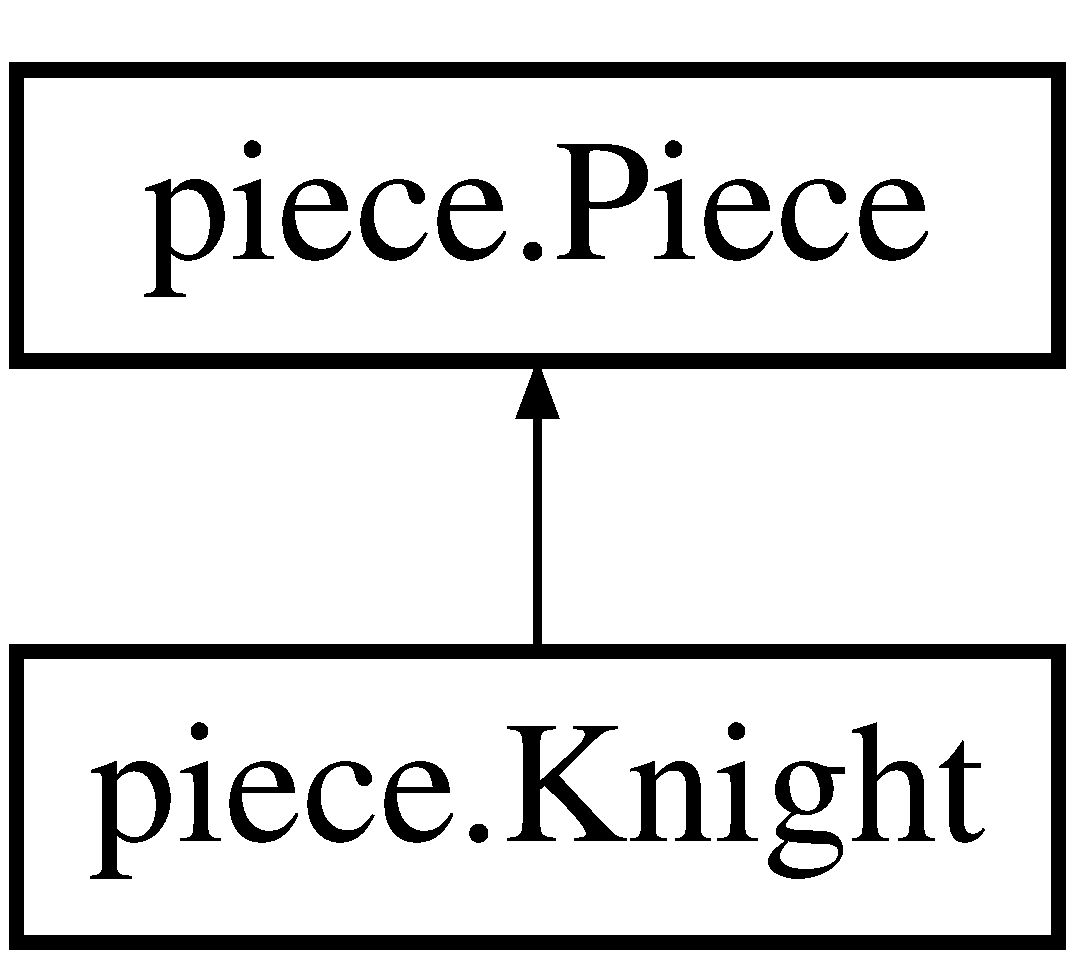
\includegraphics[height=2.000000cm]{classpiece_1_1Knight}
\end{center}
\end{figure}
\subsection*{Public Member Functions}
\begin{DoxyCompactItemize}
\item 
void \hyperlink{classpiece_1_1Knight_acb35a9cccb045988c16b1644e96e3fe7}{update\-Moves} (\hyperlink{classmodel_1_1Board}{Board} board)
\end{DoxyCompactItemize}
\subsection*{Additional Inherited Members}


\subsection{Member Function Documentation}
\hypertarget{classpiece_1_1Knight_acb35a9cccb045988c16b1644e96e3fe7}{\index{piece\-::\-Knight@{piece\-::\-Knight}!update\-Moves@{update\-Moves}}
\index{update\-Moves@{update\-Moves}!piece::Knight@{piece\-::\-Knight}}
\subsubsection[{update\-Moves}]{\setlength{\rightskip}{0pt plus 5cm}void piece.\-Knight.\-update\-Moves (
\begin{DoxyParamCaption}
\item[{{\bf Board}}]{board}
\end{DoxyParamCaption}
)\hspace{0.3cm}{\ttfamily [inline]}, {\ttfamily [virtual]}}}\label{classpiece_1_1Knight_acb35a9cccb045988c16b1644e96e3fe7}
Upates the possible moves for a given piece. 
\begin{DoxyParams}{Parameters}
{\em spaces} & The state of the chess board. \\
\hline
\end{DoxyParams}


Implements \hyperlink{classpiece_1_1Piece_a4dbb3f3506bfc5c4a2015182857d08e0}{piece.\-Piece}.



The documentation for this class was generated from the following file\-:\begin{DoxyCompactItemize}
\item 
piece/Knight.\-java\end{DoxyCompactItemize}

\hypertarget{classtest_1_1KnightTest}{\section{test.\-Knight\-Test Class Reference}
\label{classtest_1_1KnightTest}\index{test.\-Knight\-Test@{test.\-Knight\-Test}}
}
\subsection*{Public Member Functions}
\begin{DoxyCompactItemize}
\item 
\hypertarget{classtest_1_1KnightTest_a887f017cb5be7901c50d9255b840acd8}{void {\bfseries set\-Up} ()  throws Exception }\label{classtest_1_1KnightTest_a887f017cb5be7901c50d9255b840acd8}

\item 
\hypertarget{classtest_1_1KnightTest_ae51f5094ba7c3a17bc3a573635cbf9aa}{void {\bfseries knight\-Move} ()}\label{classtest_1_1KnightTest_ae51f5094ba7c3a17bc3a573635cbf9aa}

\item 
\hypertarget{classtest_1_1KnightTest_a73b0a656dec84c0b7377e8a40c1e7cb1}{void {\bfseries horizontal\-Move} ()}\label{classtest_1_1KnightTest_a73b0a656dec84c0b7377e8a40c1e7cb1}

\item 
\hypertarget{classtest_1_1KnightTest_a4b557439e93a46885846ce1996e0a1d9}{void {\bfseries vertical\-Move} ()}\label{classtest_1_1KnightTest_a4b557439e93a46885846ce1996e0a1d9}

\item 
\hypertarget{classtest_1_1KnightTest_a2763c72ea814cbcd8ce53de5b26762e7}{void {\bfseries diagonal\-Move} ()}\label{classtest_1_1KnightTest_a2763c72ea814cbcd8ce53de5b26762e7}

\item 
\hypertarget{classtest_1_1KnightTest_a78310f30261e6694da336197653e8a56}{void {\bfseries capture\-Friendly} ()}\label{classtest_1_1KnightTest_a78310f30261e6694da336197653e8a56}

\item 
\hypertarget{classtest_1_1KnightTest_a8ca0dd962c277906f726372d7fa95708}{void {\bfseries capture\-Opponent} ()}\label{classtest_1_1KnightTest_a8ca0dd962c277906f726372d7fa95708}

\item 
\hypertarget{classtest_1_1KnightTest_ab6b77c4698b4bfe88e822d9b80110dd0}{void {\bfseries jump\-Friendly} ()}\label{classtest_1_1KnightTest_ab6b77c4698b4bfe88e822d9b80110dd0}

\item 
\hypertarget{classtest_1_1KnightTest_a9e9f61589b4e1b59eb9a5fa55cff938c}{void {\bfseries jump\-Opponent} ()}\label{classtest_1_1KnightTest_a9e9f61589b4e1b59eb9a5fa55cff938c}

\end{DoxyCompactItemize}


The documentation for this class was generated from the following file\-:\begin{DoxyCompactItemize}
\item 
test/Knight\-Test.\-java\end{DoxyCompactItemize}

\hypertarget{classpiece_1_1Pawn}{\section{piece.\-Pawn Class Reference}
\label{classpiece_1_1Pawn}\index{piece.\-Pawn@{piece.\-Pawn}}
}
Inheritance diagram for piece.\-Pawn\-:\begin{figure}[H]
\begin{center}
\leavevmode
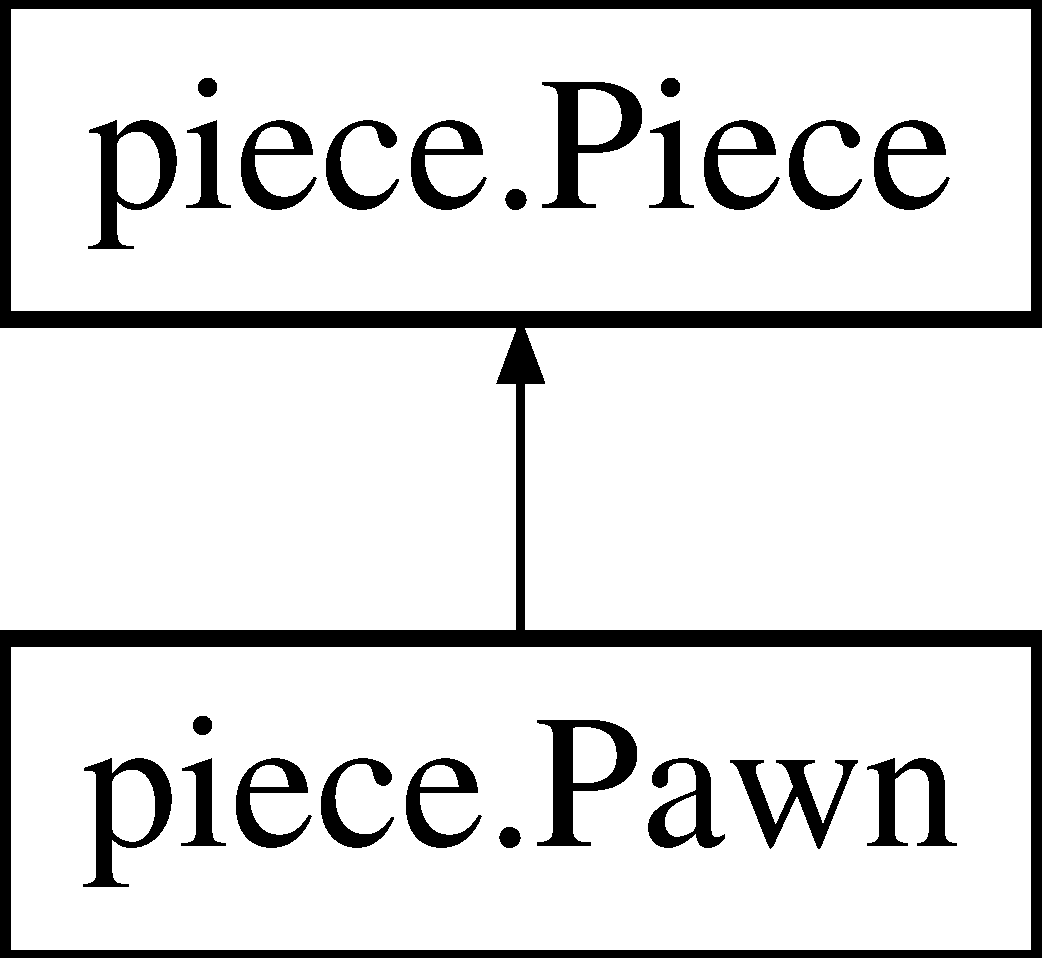
\includegraphics[height=2.000000cm]{classpiece_1_1Pawn}
\end{center}
\end{figure}
\subsection*{Public Member Functions}
\begin{DoxyCompactItemize}
\item 
void \hyperlink{classpiece_1_1Pawn_a2eaebb6e3cf4893b348bde9923a3d6cb}{update\-Moves} (\hyperlink{classmodel_1_1Board}{Board} board)
\end{DoxyCompactItemize}
\subsection*{Additional Inherited Members}


\subsection{Member Function Documentation}
\hypertarget{classpiece_1_1Pawn_a2eaebb6e3cf4893b348bde9923a3d6cb}{\index{piece\-::\-Pawn@{piece\-::\-Pawn}!update\-Moves@{update\-Moves}}
\index{update\-Moves@{update\-Moves}!piece::Pawn@{piece\-::\-Pawn}}
\subsubsection[{update\-Moves}]{\setlength{\rightskip}{0pt plus 5cm}void piece.\-Pawn.\-update\-Moves (
\begin{DoxyParamCaption}
\item[{{\bf Board}}]{board}
\end{DoxyParamCaption}
)\hspace{0.3cm}{\ttfamily [inline]}, {\ttfamily [virtual]}}}\label{classpiece_1_1Pawn_a2eaebb6e3cf4893b348bde9923a3d6cb}
Upates the possible moves for a given piece. 
\begin{DoxyParams}{Parameters}
{\em spaces} & The state of the chess board. \\
\hline
\end{DoxyParams}


Implements \hyperlink{classpiece_1_1Piece_a4dbb3f3506bfc5c4a2015182857d08e0}{piece.\-Piece}.



The documentation for this class was generated from the following file\-:\begin{DoxyCompactItemize}
\item 
piece/Pawn.\-java\end{DoxyCompactItemize}

\hypertarget{classtest_1_1PawnTest}{\section{test.\-Pawn\-Test Class Reference}
\label{classtest_1_1PawnTest}\index{test.\-Pawn\-Test@{test.\-Pawn\-Test}}
}
\subsection*{Public Member Functions}
\begin{DoxyCompactItemize}
\item 
\hypertarget{classtest_1_1PawnTest_a038138f0237a3cf3fa97277a1b598c3d}{void {\bfseries set\-Up} ()  throws Exception }\label{classtest_1_1PawnTest_a038138f0237a3cf3fa97277a1b598c3d}

\item 
\hypertarget{classtest_1_1PawnTest_abfaebd7d92927bc346a5d0503553142e}{void {\bfseries first\-Move\-Two\-Squares} ()}\label{classtest_1_1PawnTest_abfaebd7d92927bc346a5d0503553142e}

\item 
\hypertarget{classtest_1_1PawnTest_af47de7fe5148efcb861173131f31bd4d}{void {\bfseries double\-Special\-Move} ()}\label{classtest_1_1PawnTest_af47de7fe5148efcb861173131f31bd4d}

\item 
\hypertarget{classtest_1_1PawnTest_a7162a87c68676b56ca56862bc44ad627}{void {\bfseries move\-Backwards} ()}\label{classtest_1_1PawnTest_a7162a87c68676b56ca56862bc44ad627}

\item 
\hypertarget{classtest_1_1PawnTest_a0fa7bcc0e50e9a1348ae44e1aa07b546}{void {\bfseries move\-Horizontal} ()}\label{classtest_1_1PawnTest_a0fa7bcc0e50e9a1348ae44e1aa07b546}

\item 
\hypertarget{classtest_1_1PawnTest_a98796865fe2a7bbb6b1fec60db13b838}{void {\bfseries move\-Diagonal} ()}\label{classtest_1_1PawnTest_a98796865fe2a7bbb6b1fec60db13b838}

\item 
\hypertarget{classtest_1_1PawnTest_a46389bae6735e2b0bf7b00ebf6f119a6}{void {\bfseries capture\-Backwards} ()}\label{classtest_1_1PawnTest_a46389bae6735e2b0bf7b00ebf6f119a6}

\item 
\hypertarget{classtest_1_1PawnTest_a68ccfe29dcb6f2447670c19bf4dfde7a}{void {\bfseries capture\-Forwards} ()}\label{classtest_1_1PawnTest_a68ccfe29dcb6f2447670c19bf4dfde7a}

\end{DoxyCompactItemize}


The documentation for this class was generated from the following file\-:\begin{DoxyCompactItemize}
\item 
test/Pawn\-Test.\-java\end{DoxyCompactItemize}

\hypertarget{classpiece_1_1Piece}{\section{piece.\-Piece Class Reference}
\label{classpiece_1_1Piece}\index{piece.\-Piece@{piece.\-Piece}}
}
Inheritance diagram for piece.\-Piece\-:\begin{figure}[H]
\begin{center}
\leavevmode
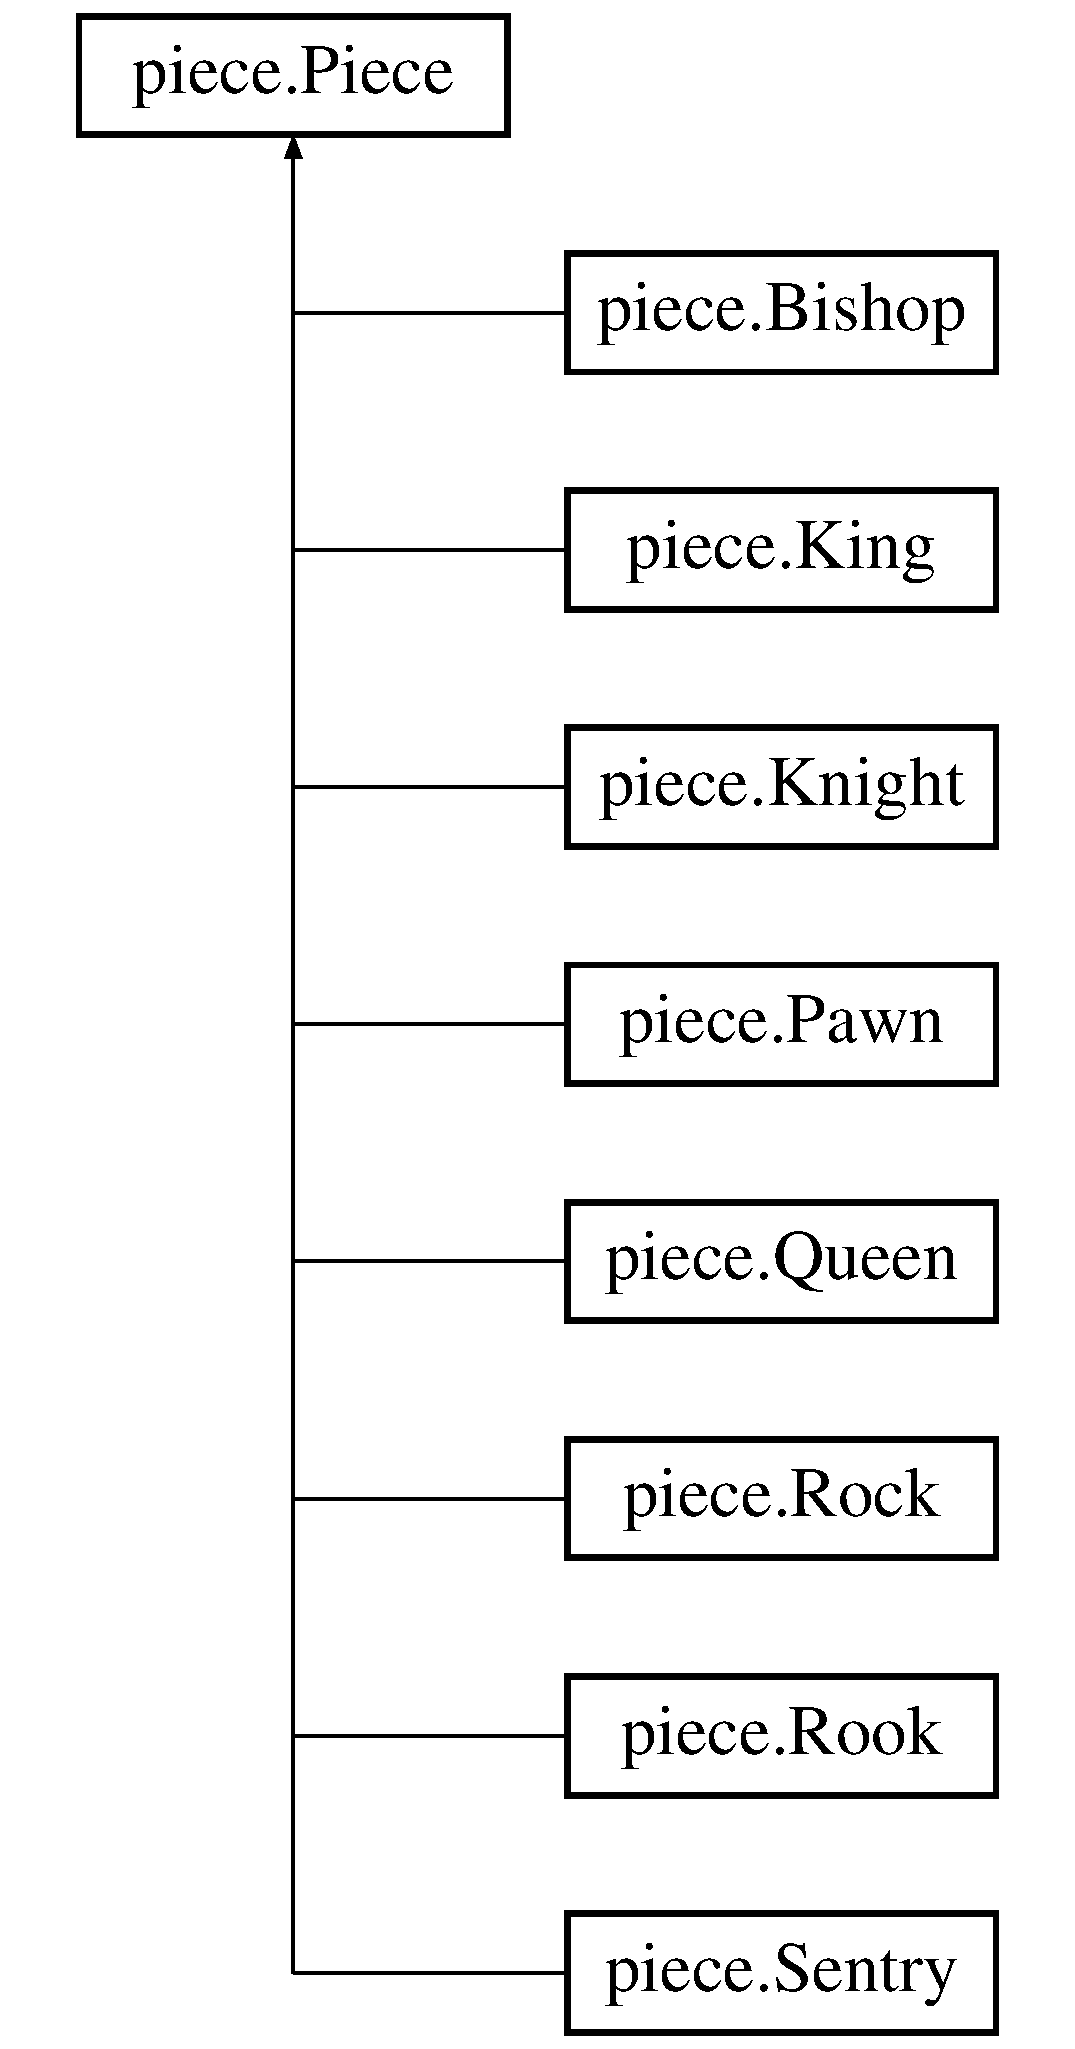
\includegraphics[height=9.000000cm]{classpiece_1_1Piece}
\end{center}
\end{figure}
\subsection*{Public Member Functions}
\begin{DoxyCompactItemize}
\item 
abstract void \hyperlink{classpiece_1_1Piece_a4dbb3f3506bfc5c4a2015182857d08e0}{update\-Moves} (\hyperlink{classmodel_1_1Board}{Board} board)
\item 
Color \hyperlink{classpiece_1_1Piece_ad4c523c97739f39df0c74059b40b24c3}{get\-Color} ()
\item 
void \hyperlink{classpiece_1_1Piece_ad1b0ab8b18993689c7bd45a9b8603bd4}{set\-Color} (Color \hyperlink{classpiece_1_1Piece_a3b9829de5683f4c966f4a6c98ad77d65}{color})
\item 
Vector$<$ \hyperlink{classmodel_1_1Space}{Space} $>$ \hyperlink{classpiece_1_1Piece_ab0a26f70a1ce3629baa8e5b13e176c9d}{get\-Moves} ()
\item 
void \hyperlink{classpiece_1_1Piece_ac9cf15e923e68e74f7a04c8108a86dab}{set\-Moves} (Vector$<$ \hyperlink{classmodel_1_1Space}{Space} $>$ \hyperlink{classpiece_1_1Piece_ab29bfb629292cb4ae39a5dd545a31aaf}{moves})
\item 
Buffered\-Image \hyperlink{classpiece_1_1Piece_afdff33667aeac45d1d9488eaeeb33cd2}{get\-Buffered\-Image} ()
\item 
void \hyperlink{classpiece_1_1Piece_a9a970552f400d8e70f2352a00a865494}{set\-Buffered\-Image} (Buffered\-Image \hyperlink{classpiece_1_1Piece_a287a5ae3797417dbc7a04def1bb8ceda}{buffered\-Image})
\item 
int \hyperlink{classpiece_1_1Piece_aa35551eff88a4a92287081afd6b16cf1}{get\-Rank} ()
\item 
void \hyperlink{classpiece_1_1Piece_a606e9a98be26e1ee783241b544c765e8}{set\-Rank} (int \hyperlink{classpiece_1_1Piece_ac015e60596ce57e3f96328fc61f66b95}{rank})
\item 
int \hyperlink{classpiece_1_1Piece_ab5386372600efab6ad744403be8ef1ad}{get\-File} ()
\item 
void \hyperlink{classpiece_1_1Piece_ad9561eda23e5bb0c595ad5db112c9d8a}{set\-File} (int \hyperlink{classpiece_1_1Piece_af30351ae20932383ee93fdd2e73f65ec}{file})
\end{DoxyCompactItemize}
\subsection*{Protected Attributes}
\begin{DoxyCompactItemize}
\item 
Color \hyperlink{classpiece_1_1Piece_a3b9829de5683f4c966f4a6c98ad77d65}{color} = null
\item 
Vector$<$ \hyperlink{classmodel_1_1Space}{Space} $>$ \hyperlink{classpiece_1_1Piece_ab29bfb629292cb4ae39a5dd545a31aaf}{moves} = null
\item 
Buffered\-Image \hyperlink{classpiece_1_1Piece_a287a5ae3797417dbc7a04def1bb8ceda}{buffered\-Image}
\item 
int \hyperlink{classpiece_1_1Piece_ac015e60596ce57e3f96328fc61f66b95}{rank}
\item 
int \hyperlink{classpiece_1_1Piece_af30351ae20932383ee93fdd2e73f65ec}{file}
\end{DoxyCompactItemize}


\subsection{Detailed Description}
\begin{DoxyAuthor}{Author}
Alex 
\end{DoxyAuthor}


\subsection{Member Function Documentation}
\hypertarget{classpiece_1_1Piece_afdff33667aeac45d1d9488eaeeb33cd2}{\index{piece\-::\-Piece@{piece\-::\-Piece}!get\-Buffered\-Image@{get\-Buffered\-Image}}
\index{get\-Buffered\-Image@{get\-Buffered\-Image}!piece::Piece@{piece\-::\-Piece}}
\subsubsection[{get\-Buffered\-Image}]{\setlength{\rightskip}{0pt plus 5cm}Buffered\-Image piece.\-Piece.\-get\-Buffered\-Image (
\begin{DoxyParamCaption}
{}
\end{DoxyParamCaption}
)\hspace{0.3cm}{\ttfamily [inline]}}}\label{classpiece_1_1Piece_afdff33667aeac45d1d9488eaeeb33cd2}
\begin{DoxyReturn}{Returns}
the buffered\-Image 
\end{DoxyReturn}
\hypertarget{classpiece_1_1Piece_ad4c523c97739f39df0c74059b40b24c3}{\index{piece\-::\-Piece@{piece\-::\-Piece}!get\-Color@{get\-Color}}
\index{get\-Color@{get\-Color}!piece::Piece@{piece\-::\-Piece}}
\subsubsection[{get\-Color}]{\setlength{\rightskip}{0pt plus 5cm}Color piece.\-Piece.\-get\-Color (
\begin{DoxyParamCaption}
{}
\end{DoxyParamCaption}
)\hspace{0.3cm}{\ttfamily [inline]}}}\label{classpiece_1_1Piece_ad4c523c97739f39df0c74059b40b24c3}
\begin{DoxyReturn}{Returns}
the color 
\end{DoxyReturn}
\hypertarget{classpiece_1_1Piece_ab5386372600efab6ad744403be8ef1ad}{\index{piece\-::\-Piece@{piece\-::\-Piece}!get\-File@{get\-File}}
\index{get\-File@{get\-File}!piece::Piece@{piece\-::\-Piece}}
\subsubsection[{get\-File}]{\setlength{\rightskip}{0pt plus 5cm}int piece.\-Piece.\-get\-File (
\begin{DoxyParamCaption}
{}
\end{DoxyParamCaption}
)\hspace{0.3cm}{\ttfamily [inline]}}}\label{classpiece_1_1Piece_ab5386372600efab6ad744403be8ef1ad}
\begin{DoxyReturn}{Returns}
the file 
\end{DoxyReturn}
\hypertarget{classpiece_1_1Piece_ab0a26f70a1ce3629baa8e5b13e176c9d}{\index{piece\-::\-Piece@{piece\-::\-Piece}!get\-Moves@{get\-Moves}}
\index{get\-Moves@{get\-Moves}!piece::Piece@{piece\-::\-Piece}}
\subsubsection[{get\-Moves}]{\setlength{\rightskip}{0pt plus 5cm}Vector$<${\bf Space}$>$ piece.\-Piece.\-get\-Moves (
\begin{DoxyParamCaption}
{}
\end{DoxyParamCaption}
)\hspace{0.3cm}{\ttfamily [inline]}}}\label{classpiece_1_1Piece_ab0a26f70a1ce3629baa8e5b13e176c9d}
\begin{DoxyReturn}{Returns}
the moves 
\end{DoxyReturn}
\hypertarget{classpiece_1_1Piece_aa35551eff88a4a92287081afd6b16cf1}{\index{piece\-::\-Piece@{piece\-::\-Piece}!get\-Rank@{get\-Rank}}
\index{get\-Rank@{get\-Rank}!piece::Piece@{piece\-::\-Piece}}
\subsubsection[{get\-Rank}]{\setlength{\rightskip}{0pt plus 5cm}int piece.\-Piece.\-get\-Rank (
\begin{DoxyParamCaption}
{}
\end{DoxyParamCaption}
)\hspace{0.3cm}{\ttfamily [inline]}}}\label{classpiece_1_1Piece_aa35551eff88a4a92287081afd6b16cf1}
\begin{DoxyReturn}{Returns}
the rank 
\end{DoxyReturn}
\hypertarget{classpiece_1_1Piece_a9a970552f400d8e70f2352a00a865494}{\index{piece\-::\-Piece@{piece\-::\-Piece}!set\-Buffered\-Image@{set\-Buffered\-Image}}
\index{set\-Buffered\-Image@{set\-Buffered\-Image}!piece::Piece@{piece\-::\-Piece}}
\subsubsection[{set\-Buffered\-Image}]{\setlength{\rightskip}{0pt plus 5cm}void piece.\-Piece.\-set\-Buffered\-Image (
\begin{DoxyParamCaption}
\item[{Buffered\-Image}]{buffered\-Image}
\end{DoxyParamCaption}
)\hspace{0.3cm}{\ttfamily [inline]}}}\label{classpiece_1_1Piece_a9a970552f400d8e70f2352a00a865494}

\begin{DoxyParams}{Parameters}
{\em buffered\-Image} & the buffered\-Image to set \\
\hline
\end{DoxyParams}
\hypertarget{classpiece_1_1Piece_ad1b0ab8b18993689c7bd45a9b8603bd4}{\index{piece\-::\-Piece@{piece\-::\-Piece}!set\-Color@{set\-Color}}
\index{set\-Color@{set\-Color}!piece::Piece@{piece\-::\-Piece}}
\subsubsection[{set\-Color}]{\setlength{\rightskip}{0pt plus 5cm}void piece.\-Piece.\-set\-Color (
\begin{DoxyParamCaption}
\item[{Color}]{color}
\end{DoxyParamCaption}
)\hspace{0.3cm}{\ttfamily [inline]}}}\label{classpiece_1_1Piece_ad1b0ab8b18993689c7bd45a9b8603bd4}

\begin{DoxyParams}{Parameters}
{\em color} & the color to set \\
\hline
\end{DoxyParams}
\hypertarget{classpiece_1_1Piece_ad9561eda23e5bb0c595ad5db112c9d8a}{\index{piece\-::\-Piece@{piece\-::\-Piece}!set\-File@{set\-File}}
\index{set\-File@{set\-File}!piece::Piece@{piece\-::\-Piece}}
\subsubsection[{set\-File}]{\setlength{\rightskip}{0pt plus 5cm}void piece.\-Piece.\-set\-File (
\begin{DoxyParamCaption}
\item[{int}]{file}
\end{DoxyParamCaption}
)\hspace{0.3cm}{\ttfamily [inline]}}}\label{classpiece_1_1Piece_ad9561eda23e5bb0c595ad5db112c9d8a}

\begin{DoxyParams}{Parameters}
{\em file} & the file to set \\
\hline
\end{DoxyParams}
\hypertarget{classpiece_1_1Piece_ac9cf15e923e68e74f7a04c8108a86dab}{\index{piece\-::\-Piece@{piece\-::\-Piece}!set\-Moves@{set\-Moves}}
\index{set\-Moves@{set\-Moves}!piece::Piece@{piece\-::\-Piece}}
\subsubsection[{set\-Moves}]{\setlength{\rightskip}{0pt plus 5cm}void piece.\-Piece.\-set\-Moves (
\begin{DoxyParamCaption}
\item[{Vector$<$ {\bf Space} $>$}]{moves}
\end{DoxyParamCaption}
)\hspace{0.3cm}{\ttfamily [inline]}}}\label{classpiece_1_1Piece_ac9cf15e923e68e74f7a04c8108a86dab}

\begin{DoxyParams}{Parameters}
{\em moves} & the moves to set \\
\hline
\end{DoxyParams}
\hypertarget{classpiece_1_1Piece_a606e9a98be26e1ee783241b544c765e8}{\index{piece\-::\-Piece@{piece\-::\-Piece}!set\-Rank@{set\-Rank}}
\index{set\-Rank@{set\-Rank}!piece::Piece@{piece\-::\-Piece}}
\subsubsection[{set\-Rank}]{\setlength{\rightskip}{0pt plus 5cm}void piece.\-Piece.\-set\-Rank (
\begin{DoxyParamCaption}
\item[{int}]{rank}
\end{DoxyParamCaption}
)\hspace{0.3cm}{\ttfamily [inline]}}}\label{classpiece_1_1Piece_a606e9a98be26e1ee783241b544c765e8}

\begin{DoxyParams}{Parameters}
{\em rank} & the rank to set \\
\hline
\end{DoxyParams}
\hypertarget{classpiece_1_1Piece_a4dbb3f3506bfc5c4a2015182857d08e0}{\index{piece\-::\-Piece@{piece\-::\-Piece}!update\-Moves@{update\-Moves}}
\index{update\-Moves@{update\-Moves}!piece::Piece@{piece\-::\-Piece}}
\subsubsection[{update\-Moves}]{\setlength{\rightskip}{0pt plus 5cm}abstract void piece.\-Piece.\-update\-Moves (
\begin{DoxyParamCaption}
\item[{{\bf Board}}]{board}
\end{DoxyParamCaption}
)\hspace{0.3cm}{\ttfamily [pure virtual]}}}\label{classpiece_1_1Piece_a4dbb3f3506bfc5c4a2015182857d08e0}
Upates the possible moves for a given piece. 
\begin{DoxyParams}{Parameters}
{\em spaces} & The state of the chess board. \\
\hline
\end{DoxyParams}


Implemented in \hyperlink{classpiece_1_1Knight_acb35a9cccb045988c16b1644e96e3fe7}{piece.\-Knight}, \hyperlink{classpiece_1_1Rock_a29ae1213c1bc15174d0cffc875255535}{piece.\-Rock}, \hyperlink{classpiece_1_1Bishop_af3af2a374601e579cd5249b7951f0c81}{piece.\-Bishop}, \hyperlink{classpiece_1_1King_a93304e2c4a5b94acc2c4606a9d2a9f4e}{piece.\-King}, \hyperlink{classpiece_1_1Rook_a2f406a5c22d688b22ce1f5485a83a3ba}{piece.\-Rook}, \hyperlink{classpiece_1_1Queen_aee4df922b394e55464f07f60e7b98c3c}{piece.\-Queen}, \hyperlink{classpiece_1_1Pawn_a2eaebb6e3cf4893b348bde9923a3d6cb}{piece.\-Pawn}, and \hyperlink{classpiece_1_1Sentry_adfcb33eac6e929b960ad991cd073bf5e}{piece.\-Sentry}.



\subsection{Member Data Documentation}
\hypertarget{classpiece_1_1Piece_a287a5ae3797417dbc7a04def1bb8ceda}{\index{piece\-::\-Piece@{piece\-::\-Piece}!buffered\-Image@{buffered\-Image}}
\index{buffered\-Image@{buffered\-Image}!piece::Piece@{piece\-::\-Piece}}
\subsubsection[{buffered\-Image}]{\setlength{\rightskip}{0pt plus 5cm}Buffered\-Image piece.\-Piece.\-buffered\-Image\hspace{0.3cm}{\ttfamily [protected]}}}\label{classpiece_1_1Piece_a287a5ae3797417dbc7a04def1bb8ceda}
The buffered\-Image of a piece \hypertarget{classpiece_1_1Piece_a3b9829de5683f4c966f4a6c98ad77d65}{\index{piece\-::\-Piece@{piece\-::\-Piece}!color@{color}}
\index{color@{color}!piece::Piece@{piece\-::\-Piece}}
\subsubsection[{color}]{\setlength{\rightskip}{0pt plus 5cm}Color piece.\-Piece.\-color = null\hspace{0.3cm}{\ttfamily [protected]}}}\label{classpiece_1_1Piece_a3b9829de5683f4c966f4a6c98ad77d65}

\begin{DoxyParams}{Parameters}
{\em color} & \\
\hline
{\em moves} & \\
\hline
{\em buffered\-Image} & \\
\hline
{\em rank} & \\
\hline
{\em file} & The color of a piece. (B\-L\-A\-C\-K, W\-H\-I\-T\-E, N\-U\-L\-L) \\
\hline
\end{DoxyParams}
\hypertarget{classpiece_1_1Piece_af30351ae20932383ee93fdd2e73f65ec}{\index{piece\-::\-Piece@{piece\-::\-Piece}!file@{file}}
\index{file@{file}!piece::Piece@{piece\-::\-Piece}}
\subsubsection[{file}]{\setlength{\rightskip}{0pt plus 5cm}int piece.\-Piece.\-file\hspace{0.3cm}{\ttfamily [protected]}}}\label{classpiece_1_1Piece_af30351ae20932383ee93fdd2e73f65ec}
file of piece \hypertarget{classpiece_1_1Piece_ab29bfb629292cb4ae39a5dd545a31aaf}{\index{piece\-::\-Piece@{piece\-::\-Piece}!moves@{moves}}
\index{moves@{moves}!piece::Piece@{piece\-::\-Piece}}
\subsubsection[{moves}]{\setlength{\rightskip}{0pt plus 5cm}Vector$<${\bf Space}$>$ piece.\-Piece.\-moves = null\hspace{0.3cm}{\ttfamily [protected]}}}\label{classpiece_1_1Piece_ab29bfb629292cb4ae39a5dd545a31aaf}
The possible moves for a piece. \hypertarget{classpiece_1_1Piece_ac015e60596ce57e3f96328fc61f66b95}{\index{piece\-::\-Piece@{piece\-::\-Piece}!rank@{rank}}
\index{rank@{rank}!piece::Piece@{piece\-::\-Piece}}
\subsubsection[{rank}]{\setlength{\rightskip}{0pt plus 5cm}int piece.\-Piece.\-rank\hspace{0.3cm}{\ttfamily [protected]}}}\label{classpiece_1_1Piece_ac015e60596ce57e3f96328fc61f66b95}
rank of piece 

The documentation for this class was generated from the following file\-:\begin{DoxyCompactItemize}
\item 
piece/Piece.\-java\end{DoxyCompactItemize}

\hypertarget{classlogic_1_1PieceLogic}{\section{logic.\-Piece\-Logic Class Reference}
\label{classlogic_1_1PieceLogic}\index{logic.\-Piece\-Logic@{logic.\-Piece\-Logic}}
}
\subsection*{Static Public Member Functions}
\begin{DoxyCompactItemize}
\item 
static boolean \hyperlink{classlogic_1_1PieceLogic_aac7446d10b195afb378411addcf5b93a}{is\-Valid\-Move} (\hyperlink{classpiece_1_1Piece}{Piece} piece, int rank, int file)
\item 
static boolean \hyperlink{classlogic_1_1PieceLogic_a93161b8617563e7e01657c47e63187db}{same\-Owner} (\hyperlink{classpiece_1_1Piece}{Piece} piece, \hyperlink{classpiece_1_1Piece}{Piece} other)
\item 
static \hyperlink{classpiece_1_1Piece}{Piece} \hyperlink{classlogic_1_1PieceLogic_a82d3489e7f023e7248abab45768ecf45}{set\-Up\-Piece} (\hyperlink{classpiece_1_1Piece}{Piece} piece, Color player)
\item 
\hypertarget{classlogic_1_1PieceLogic_ae9554b341dd00ca6bc8ec352225276c4}{static \hyperlink{classpiece_1_1Piece}{Piece} {\bfseries copy\-Piece} (\hyperlink{classpiece_1_1Piece}{Piece} piece, \hyperlink{classpiece_1_1Piece}{Piece} other)}\label{classlogic_1_1PieceLogic_ae9554b341dd00ca6bc8ec352225276c4}

\item 
static boolean \hyperlink{classlogic_1_1PieceLogic_a89579badd601a4707cd3a45ee7934bf0}{add\-Move} (\hyperlink{classpiece_1_1Piece}{Piece} piece, \hyperlink{classpiece_1_1Piece}{Piece} cur\-Space, int rank, int file)
\item 
static Buffered\-Image \hyperlink{classlogic_1_1PieceLogic_a25890c82076e10599f19590780feb29c}{get\-Piece\-Image} (\hyperlink{classpiece_1_1Piece}{Piece} piece)
\end{DoxyCompactItemize}


\subsection{Member Function Documentation}
\hypertarget{classlogic_1_1PieceLogic_a89579badd601a4707cd3a45ee7934bf0}{\index{logic\-::\-Piece\-Logic@{logic\-::\-Piece\-Logic}!add\-Move@{add\-Move}}
\index{add\-Move@{add\-Move}!logic::PieceLogic@{logic\-::\-Piece\-Logic}}
\subsubsection[{add\-Move}]{\setlength{\rightskip}{0pt plus 5cm}static boolean logic.\-Piece\-Logic.\-add\-Move (
\begin{DoxyParamCaption}
\item[{{\bf Piece}}]{piece, }
\item[{{\bf Piece}}]{cur\-Space, }
\item[{int}]{rank, }
\item[{int}]{file}
\end{DoxyParamCaption}
)\hspace{0.3cm}{\ttfamily [inline]}, {\ttfamily [static]}}}\label{classlogic_1_1PieceLogic_a89579badd601a4707cd3a45ee7934bf0}
Update\-Moves helper that checks if a given square should be added. It must not have the same owner or \begin{DoxyReturn}{Returns}
true if the piece cannot jump past the square 
\end{DoxyReturn}
\hypertarget{classlogic_1_1PieceLogic_a25890c82076e10599f19590780feb29c}{\index{logic\-::\-Piece\-Logic@{logic\-::\-Piece\-Logic}!get\-Piece\-Image@{get\-Piece\-Image}}
\index{get\-Piece\-Image@{get\-Piece\-Image}!logic::PieceLogic@{logic\-::\-Piece\-Logic}}
\subsubsection[{get\-Piece\-Image}]{\setlength{\rightskip}{0pt plus 5cm}static Buffered\-Image logic.\-Piece\-Logic.\-get\-Piece\-Image (
\begin{DoxyParamCaption}
\item[{{\bf Piece}}]{piece}
\end{DoxyParamCaption}
)\hspace{0.3cm}{\ttfamily [inline]}, {\ttfamily [static]}}}\label{classlogic_1_1PieceLogic_a25890c82076e10599f19590780feb29c}
\begin{DoxyReturn}{Returns}
the image file on disk representing the piece 
\end{DoxyReturn}
\hypertarget{classlogic_1_1PieceLogic_aac7446d10b195afb378411addcf5b93a}{\index{logic\-::\-Piece\-Logic@{logic\-::\-Piece\-Logic}!is\-Valid\-Move@{is\-Valid\-Move}}
\index{is\-Valid\-Move@{is\-Valid\-Move}!logic::PieceLogic@{logic\-::\-Piece\-Logic}}
\subsubsection[{is\-Valid\-Move}]{\setlength{\rightskip}{0pt plus 5cm}static boolean logic.\-Piece\-Logic.\-is\-Valid\-Move (
\begin{DoxyParamCaption}
\item[{{\bf Piece}}]{piece, }
\item[{int}]{rank, }
\item[{int}]{file}
\end{DoxyParamCaption}
)\hspace{0.3cm}{\ttfamily [inline]}, {\ttfamily [static]}}}\label{classlogic_1_1PieceLogic_aac7446d10b195afb378411addcf5b93a}

\begin{DoxyParams}{Parameters}
{\em target} & the (rank,file) pair on the board to move to \\
\hline
\end{DoxyParams}
\begin{DoxyReturn}{Returns}
true if a given move is possible for a piece 
\end{DoxyReturn}
\hypertarget{classlogic_1_1PieceLogic_a93161b8617563e7e01657c47e63187db}{\index{logic\-::\-Piece\-Logic@{logic\-::\-Piece\-Logic}!same\-Owner@{same\-Owner}}
\index{same\-Owner@{same\-Owner}!logic::PieceLogic@{logic\-::\-Piece\-Logic}}
\subsubsection[{same\-Owner}]{\setlength{\rightskip}{0pt plus 5cm}static boolean logic.\-Piece\-Logic.\-same\-Owner (
\begin{DoxyParamCaption}
\item[{{\bf Piece}}]{piece, }
\item[{{\bf Piece}}]{other}
\end{DoxyParamCaption}
)\hspace{0.3cm}{\ttfamily [inline]}, {\ttfamily [static]}}}\label{classlogic_1_1PieceLogic_a93161b8617563e7e01657c47e63187db}

\begin{DoxyParams}{Parameters}
{\em other} & the piece to compare the current one with \\
\hline
\end{DoxyParams}
\begin{DoxyReturn}{Returns}
true if one piece has the same owner as the other 
\end{DoxyReturn}
\hypertarget{classlogic_1_1PieceLogic_a82d3489e7f023e7248abab45768ecf45}{\index{logic\-::\-Piece\-Logic@{logic\-::\-Piece\-Logic}!set\-Up\-Piece@{set\-Up\-Piece}}
\index{set\-Up\-Piece@{set\-Up\-Piece}!logic::PieceLogic@{logic\-::\-Piece\-Logic}}
\subsubsection[{set\-Up\-Piece}]{\setlength{\rightskip}{0pt plus 5cm}static {\bf Piece} logic.\-Piece\-Logic.\-set\-Up\-Piece (
\begin{DoxyParamCaption}
\item[{{\bf Piece}}]{piece, }
\item[{Color}]{player}
\end{DoxyParamCaption}
)\hspace{0.3cm}{\ttfamily [inline]}, {\ttfamily [static]}}}\label{classlogic_1_1PieceLogic_a82d3489e7f023e7248abab45768ecf45}
Converts a string to an instance of a new piece. 
\begin{DoxyParams}{Parameters}
{\em piece} & the type of piece to instantiate \\
\hline
{\em player} & the color of piece to initialize \\
\hline
\end{DoxyParams}
\begin{DoxyReturn}{Returns}
the initialized piece matching the string input 
\end{DoxyReturn}


The documentation for this class was generated from the following file\-:\begin{DoxyCompactItemize}
\item 
logic/Piece\-Logic.\-java\end{DoxyCompactItemize}

\hypertarget{classtest_1_1PieceTest}{\section{test.\-Piece\-Test Class Reference}
\label{classtest_1_1PieceTest}\index{test.\-Piece\-Test@{test.\-Piece\-Test}}
}
\subsection*{Public Member Functions}
\begin{DoxyCompactItemize}
\item 
\hypertarget{classtest_1_1PieceTest_aa78f2de63d4382124aeb5cb18d20c818}{void {\bfseries set\-Up} ()  throws Exception }\label{classtest_1_1PieceTest_aa78f2de63d4382124aeb5cb18d20c818}

\item 
\hypertarget{classtest_1_1PieceTest_aace405af329ed34874c831ad48dd95c7}{void {\bfseries outof\-Bounds\-Set\-Piece} ()}\label{classtest_1_1PieceTest_aace405af329ed34874c831ad48dd95c7}

\item 
\hypertarget{classtest_1_1PieceTest_a02be3c2128dbece1a39e6a5e0f97843d}{void {\bfseries valid\-Set\-Piece} ()}\label{classtest_1_1PieceTest_a02be3c2128dbece1a39e6a5e0f97843d}

\item 
\hypertarget{classtest_1_1PieceTest_a1505849f17d2e6749d1b7a4bcab01515}{void {\bfseries double\-Set\-Piece} ()}\label{classtest_1_1PieceTest_a1505849f17d2e6749d1b7a4bcab01515}

\item 
\hypertarget{classtest_1_1PieceTest_af8ddb64c7bdfbdd3935fa25c9cca165f}{void {\bfseries empty\-Piece\-Move} ()}\label{classtest_1_1PieceTest_af8ddb64c7bdfbdd3935fa25c9cca165f}

\end{DoxyCompactItemize}


The documentation for this class was generated from the following file\-:\begin{DoxyCompactItemize}
\item 
test/Piece\-Test.\-java\end{DoxyCompactItemize}

\hypertarget{classcontroller_1_1Player}{\section{controller.\-Player Class Reference}
\label{classcontroller_1_1Player}\index{controller.\-Player@{controller.\-Player}}
}
\subsection*{Public Member Functions}
\begin{DoxyCompactItemize}
\item 
\hypertarget{classcontroller_1_1Player_a58bbebdd3aa47ede2185c45224678993}{{\bfseries Player} (String name, Color piece\-Color, boolean move\-First)}\label{classcontroller_1_1Player_a58bbebdd3aa47ede2185c45224678993}

\item 
\hypertarget{classcontroller_1_1Player_a78ec50c3386297a1259b708256f84cdc}{Color {\bfseries change\-Color} (Color curr\-Color)}\label{classcontroller_1_1Player_a78ec50c3386297a1259b708256f84cdc}

\end{DoxyCompactItemize}
\subsection*{Public Attributes}
\begin{DoxyCompactItemize}
\item 
\hypertarget{classcontroller_1_1Player_a2ad925eb3b21c1775d67a9a2d37b1f5d}{String {\bfseries name}}\label{classcontroller_1_1Player_a2ad925eb3b21c1775d67a9a2d37b1f5d}

\item 
\hypertarget{classcontroller_1_1Player_a239bc3aadcce4cb775af2a7add5b23db}{Color {\bfseries piece\-Color}}\label{classcontroller_1_1Player_a239bc3aadcce4cb775af2a7add5b23db}

\item 
\hypertarget{classcontroller_1_1Player_a52e9c6b60ae75a34e37757e212419d89}{int {\bfseries score}}\label{classcontroller_1_1Player_a52e9c6b60ae75a34e37757e212419d89}

\item 
\hypertarget{classcontroller_1_1Player_a1f90db3dc9aeb4f8861177b5546459f5}{boolean {\bfseries move\-First}}\label{classcontroller_1_1Player_a1f90db3dc9aeb4f8861177b5546459f5}

\end{DoxyCompactItemize}


The documentation for this class was generated from the following file\-:\begin{DoxyCompactItemize}
\item 
controller/Player.\-java\end{DoxyCompactItemize}

\hypertarget{classpiece_1_1Queen}{\section{piece.\-Queen Class Reference}
\label{classpiece_1_1Queen}\index{piece.\-Queen@{piece.\-Queen}}
}
Inheritance diagram for piece.\-Queen\-:\begin{figure}[H]
\begin{center}
\leavevmode
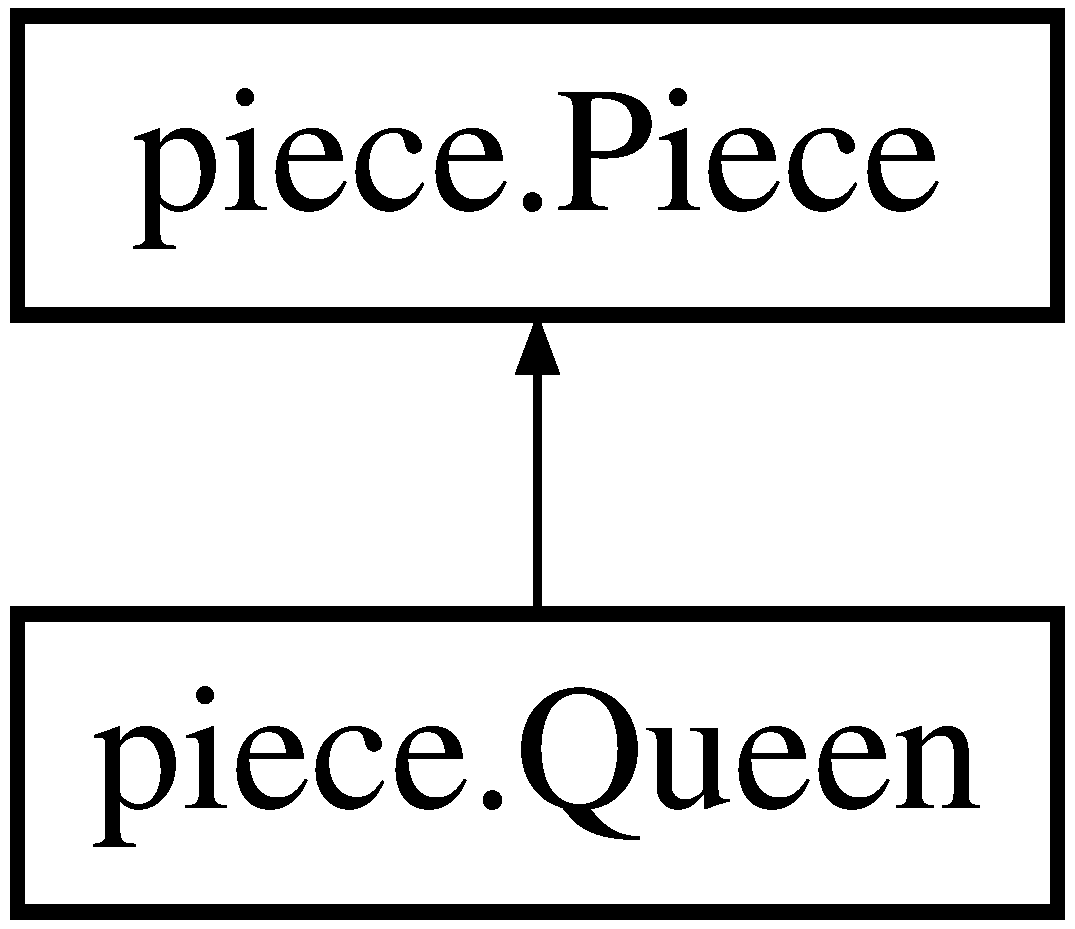
\includegraphics[height=2.000000cm]{classpiece_1_1Queen}
\end{center}
\end{figure}
\subsection*{Public Member Functions}
\begin{DoxyCompactItemize}
\item 
void \hyperlink{classpiece_1_1Queen_aee4df922b394e55464f07f60e7b98c3c}{update\-Moves} (\hyperlink{classmodel_1_1Board}{Board} board)
\end{DoxyCompactItemize}
\subsection*{Additional Inherited Members}


\subsection{Member Function Documentation}
\hypertarget{classpiece_1_1Queen_aee4df922b394e55464f07f60e7b98c3c}{\index{piece\-::\-Queen@{piece\-::\-Queen}!update\-Moves@{update\-Moves}}
\index{update\-Moves@{update\-Moves}!piece::Queen@{piece\-::\-Queen}}
\subsubsection[{update\-Moves}]{\setlength{\rightskip}{0pt plus 5cm}void piece.\-Queen.\-update\-Moves (
\begin{DoxyParamCaption}
\item[{{\bf Board}}]{board}
\end{DoxyParamCaption}
)\hspace{0.3cm}{\ttfamily [inline]}, {\ttfamily [virtual]}}}\label{classpiece_1_1Queen_aee4df922b394e55464f07f60e7b98c3c}
Upates the possible moves for a given piece. 
\begin{DoxyParams}{Parameters}
{\em spaces} & The state of the chess board. \\
\hline
\end{DoxyParams}


Implements \hyperlink{classpiece_1_1Piece_a4dbb3f3506bfc5c4a2015182857d08e0}{piece.\-Piece}.



The documentation for this class was generated from the following file\-:\begin{DoxyCompactItemize}
\item 
piece/Queen.\-java\end{DoxyCompactItemize}

\hypertarget{classtest_1_1QueenTest}{\section{test.\-Queen\-Test Class Reference}
\label{classtest_1_1QueenTest}\index{test.\-Queen\-Test@{test.\-Queen\-Test}}
}
\subsection*{Public Member Functions}
\begin{DoxyCompactItemize}
\item 
\hypertarget{classtest_1_1QueenTest_a2fd72a88b7be3bdd030673c393b1ba3c}{void {\bfseries set\-Up} ()  throws Exception }\label{classtest_1_1QueenTest_a2fd72a88b7be3bdd030673c393b1ba3c}

\item 
\hypertarget{classtest_1_1QueenTest_ae2e18652724a455899eae0b05488f079}{void {\bfseries diagonal\-Move} ()}\label{classtest_1_1QueenTest_ae2e18652724a455899eae0b05488f079}

\item 
\hypertarget{classtest_1_1QueenTest_a6cc3974c0bc994678b1c87ec31962517}{void {\bfseries horizontal\-Move} ()}\label{classtest_1_1QueenTest_a6cc3974c0bc994678b1c87ec31962517}

\item 
\hypertarget{classtest_1_1QueenTest_ad3cf5a884cc6abf99e95f1c36cfd9d98}{void {\bfseries vertical\-Move} ()}\label{classtest_1_1QueenTest_ad3cf5a884cc6abf99e95f1c36cfd9d98}

\item 
\hypertarget{classtest_1_1QueenTest_a2b4448ad0a46824aeeb8c01d3288a4d7}{void {\bfseries wierd\-Move} ()}\label{classtest_1_1QueenTest_a2b4448ad0a46824aeeb8c01d3288a4d7}

\item 
\hypertarget{classtest_1_1QueenTest_a60628e3cff15dc718bf4a56c0bab1b53}{void {\bfseries capture\-Friendly} ()}\label{classtest_1_1QueenTest_a60628e3cff15dc718bf4a56c0bab1b53}

\item 
\hypertarget{classtest_1_1QueenTest_a0dd5be7a9256654cfa1157040839af9e}{void {\bfseries capture\-Opponent} ()}\label{classtest_1_1QueenTest_a0dd5be7a9256654cfa1157040839af9e}

\item 
\hypertarget{classtest_1_1QueenTest_a6f7a8e2c4eb0417bcbcf12c350e03497}{void {\bfseries jump\-Friendly} ()}\label{classtest_1_1QueenTest_a6f7a8e2c4eb0417bcbcf12c350e03497}

\item 
\hypertarget{classtest_1_1QueenTest_aa9522b9d50934a02503d262ccca33d09}{void {\bfseries jump\-Enemy} ()}\label{classtest_1_1QueenTest_aa9522b9d50934a02503d262ccca33d09}

\end{DoxyCompactItemize}


The documentation for this class was generated from the following file\-:\begin{DoxyCompactItemize}
\item 
test/Queen\-Test.\-java\end{DoxyCompactItemize}

\hypertarget{classpiece_1_1Rock}{\section{piece.\-Rock Class Reference}
\label{classpiece_1_1Rock}\index{piece.\-Rock@{piece.\-Rock}}
}
Inheritance diagram for piece.\-Rock\-:\begin{figure}[H]
\begin{center}
\leavevmode
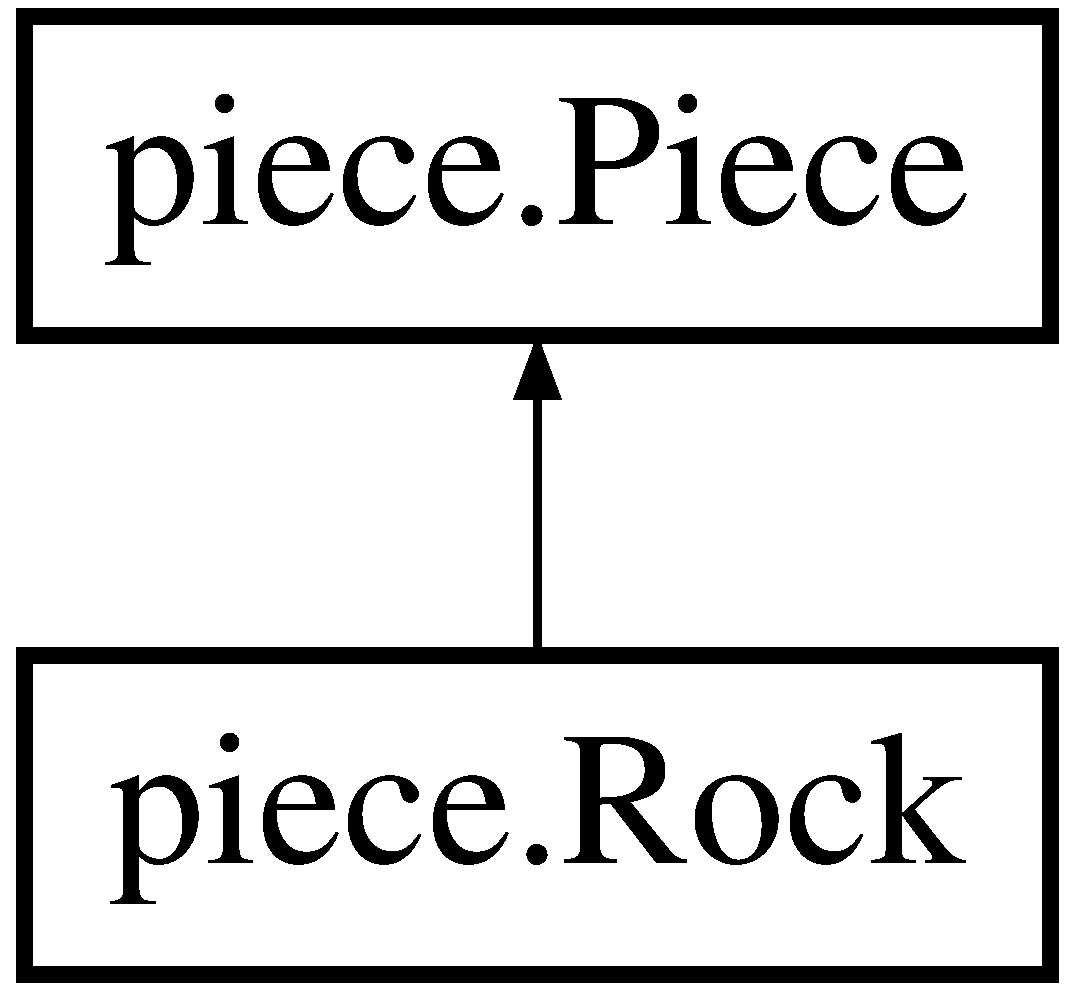
\includegraphics[height=2.000000cm]{classpiece_1_1Rock}
\end{center}
\end{figure}
\subsection*{Public Member Functions}
\begin{DoxyCompactItemize}
\item 
void \hyperlink{classpiece_1_1Rock_a29ae1213c1bc15174d0cffc875255535}{update\-Moves} (\hyperlink{classmodel_1_1Board}{Board} board)
\end{DoxyCompactItemize}
\subsection*{Additional Inherited Members}


\subsection{Member Function Documentation}
\hypertarget{classpiece_1_1Rock_a29ae1213c1bc15174d0cffc875255535}{\index{piece\-::\-Rock@{piece\-::\-Rock}!update\-Moves@{update\-Moves}}
\index{update\-Moves@{update\-Moves}!piece::Rock@{piece\-::\-Rock}}
\subsubsection[{update\-Moves}]{\setlength{\rightskip}{0pt plus 5cm}void piece.\-Rock.\-update\-Moves (
\begin{DoxyParamCaption}
\item[{{\bf Board}}]{board}
\end{DoxyParamCaption}
)\hspace{0.3cm}{\ttfamily [inline]}, {\ttfamily [virtual]}}}\label{classpiece_1_1Rock_a29ae1213c1bc15174d0cffc875255535}
Upates the possible moves for a given piece. 
\begin{DoxyParams}{Parameters}
{\em spaces} & The state of the chess board. \\
\hline
\end{DoxyParams}


Implements \hyperlink{classpiece_1_1Piece_a4dbb3f3506bfc5c4a2015182857d08e0}{piece.\-Piece}.



The documentation for this class was generated from the following file\-:\begin{DoxyCompactItemize}
\item 
piece/Rock.\-java\end{DoxyCompactItemize}

\hypertarget{classtest_1_1RockTest}{\section{test.\-Rock\-Test Class Reference}
\label{classtest_1_1RockTest}\index{test.\-Rock\-Test@{test.\-Rock\-Test}}
}
\subsection*{Public Member Functions}
\begin{DoxyCompactItemize}
\item 
\hypertarget{classtest_1_1RockTest_a1d8c12b4b9c99dca528ffb0f8d91a40e}{void {\bfseries set\-Up} ()  throws Exception }\label{classtest_1_1RockTest_a1d8c12b4b9c99dca528ffb0f8d91a40e}

\item 
\hypertarget{classtest_1_1RockTest_a29ef94577334161340abc4488b7ca165}{void {\bfseries set\-Rock} ()}\label{classtest_1_1RockTest_a29ef94577334161340abc4488b7ca165}

\item 
\hypertarget{classtest_1_1RockTest_af23c2609070b15ffb6893ba1e6024e0a}{void {\bfseries cant\-Move} ()}\label{classtest_1_1RockTest_af23c2609070b15ffb6893ba1e6024e0a}

\end{DoxyCompactItemize}


The documentation for this class was generated from the following file\-:\begin{DoxyCompactItemize}
\item 
test/Rock\-Test.\-java\end{DoxyCompactItemize}

\hypertarget{classpiece_1_1Rook}{\section{piece.\-Rook Class Reference}
\label{classpiece_1_1Rook}\index{piece.\-Rook@{piece.\-Rook}}
}
Inheritance diagram for piece.\-Rook\-:\begin{figure}[H]
\begin{center}
\leavevmode
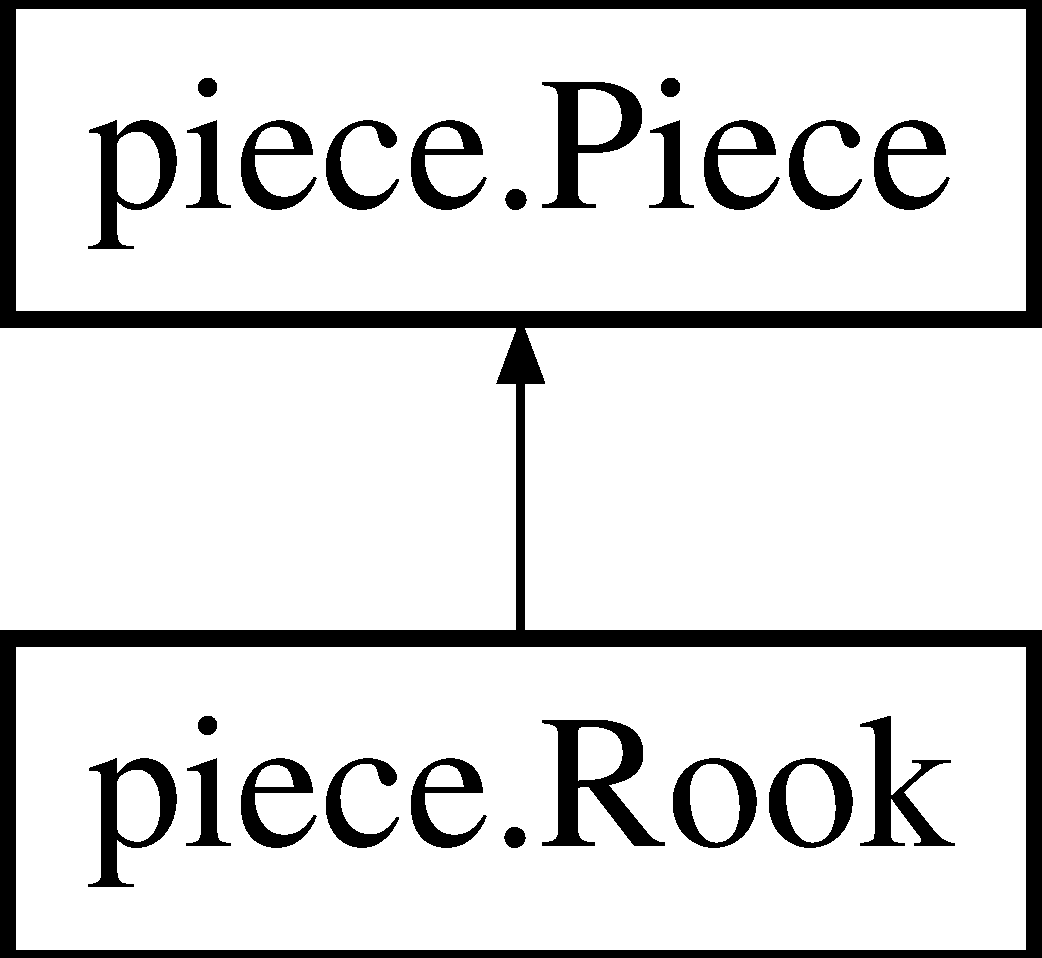
\includegraphics[height=2.000000cm]{classpiece_1_1Rook}
\end{center}
\end{figure}
\subsection*{Public Member Functions}
\begin{DoxyCompactItemize}
\item 
void \hyperlink{classpiece_1_1Rook_a2f406a5c22d688b22ce1f5485a83a3ba}{update\-Moves} (\hyperlink{classmodel_1_1Board}{Board} board)
\end{DoxyCompactItemize}
\subsection*{Additional Inherited Members}


\subsection{Member Function Documentation}
\hypertarget{classpiece_1_1Rook_a2f406a5c22d688b22ce1f5485a83a3ba}{\index{piece\-::\-Rook@{piece\-::\-Rook}!update\-Moves@{update\-Moves}}
\index{update\-Moves@{update\-Moves}!piece::Rook@{piece\-::\-Rook}}
\subsubsection[{update\-Moves}]{\setlength{\rightskip}{0pt plus 5cm}void piece.\-Rook.\-update\-Moves (
\begin{DoxyParamCaption}
\item[{{\bf Board}}]{board}
\end{DoxyParamCaption}
)\hspace{0.3cm}{\ttfamily [inline]}, {\ttfamily [virtual]}}}\label{classpiece_1_1Rook_a2f406a5c22d688b22ce1f5485a83a3ba}
Upates the possible moves for a given piece. 
\begin{DoxyParams}{Parameters}
{\em spaces} & The state of the chess board. \\
\hline
\end{DoxyParams}


Implements \hyperlink{classpiece_1_1Piece_a4dbb3f3506bfc5c4a2015182857d08e0}{piece.\-Piece}.



The documentation for this class was generated from the following file\-:\begin{DoxyCompactItemize}
\item 
piece/Rook.\-java\end{DoxyCompactItemize}

\hypertarget{classtest_1_1RookTest}{\section{test.\-Rook\-Test Class Reference}
\label{classtest_1_1RookTest}\index{test.\-Rook\-Test@{test.\-Rook\-Test}}
}
\subsection*{Public Member Functions}
\begin{DoxyCompactItemize}
\item 
\hypertarget{classtest_1_1RookTest_add7be25aaf699f5602967c05afd1c440}{void {\bfseries set\-Up} ()  throws Exception }\label{classtest_1_1RookTest_add7be25aaf699f5602967c05afd1c440}

\item 
\hypertarget{classtest_1_1RookTest_a00f59be72d5e77c1031869173b367501}{void {\bfseries rook\-Move} ()}\label{classtest_1_1RookTest_a00f59be72d5e77c1031869173b367501}

\item 
\hypertarget{classtest_1_1RookTest_a51b0a931ae05c14967e0f12651f22108}{void {\bfseries out\-Of\-Bounds\-Move} ()}\label{classtest_1_1RookTest_a51b0a931ae05c14967e0f12651f22108}

\item 
\hypertarget{classtest_1_1RookTest_ad28cda0fc3b7ee0b496d6f83ed4b4378}{void {\bfseries diagonal\-Move} ()}\label{classtest_1_1RookTest_ad28cda0fc3b7ee0b496d6f83ed4b4378}

\item 
\hypertarget{classtest_1_1RookTest_a4df3d93b31c6f0774d51e6b1d37e70d4}{void {\bfseries weird\-Move} ()}\label{classtest_1_1RookTest_a4df3d93b31c6f0774d51e6b1d37e70d4}

\item 
\hypertarget{classtest_1_1RookTest_a350c9419e97f25750cb46c0300db7bed}{void {\bfseries capture\-Friendly} ()}\label{classtest_1_1RookTest_a350c9419e97f25750cb46c0300db7bed}

\item 
\hypertarget{classtest_1_1RookTest_a2ff3d4caae74d28c3011abf63d3ce4b5}{void {\bfseries capture\-Opponent} ()}\label{classtest_1_1RookTest_a2ff3d4caae74d28c3011abf63d3ce4b5}

\item 
\hypertarget{classtest_1_1RookTest_adb47a16b06bc068c3b7188565bba960b}{void {\bfseries jump\-Friendly\-Pieces} ()}\label{classtest_1_1RookTest_adb47a16b06bc068c3b7188565bba960b}

\item 
\hypertarget{classtest_1_1RookTest_a71ecc84ed26f7ef40f5d3bbcd87a42a9}{void {\bfseries jump\-Enemy\-Piece} ()}\label{classtest_1_1RookTest_a71ecc84ed26f7ef40f5d3bbcd87a42a9}

\end{DoxyCompactItemize}


The documentation for this class was generated from the following file\-:\begin{DoxyCompactItemize}
\item 
test/Rook\-Test.\-java\end{DoxyCompactItemize}

\hypertarget{classpiece_1_1Sentry}{\section{piece.\-Sentry Class Reference}
\label{classpiece_1_1Sentry}\index{piece.\-Sentry@{piece.\-Sentry}}
}
Inheritance diagram for piece.\-Sentry\-:\begin{figure}[H]
\begin{center}
\leavevmode
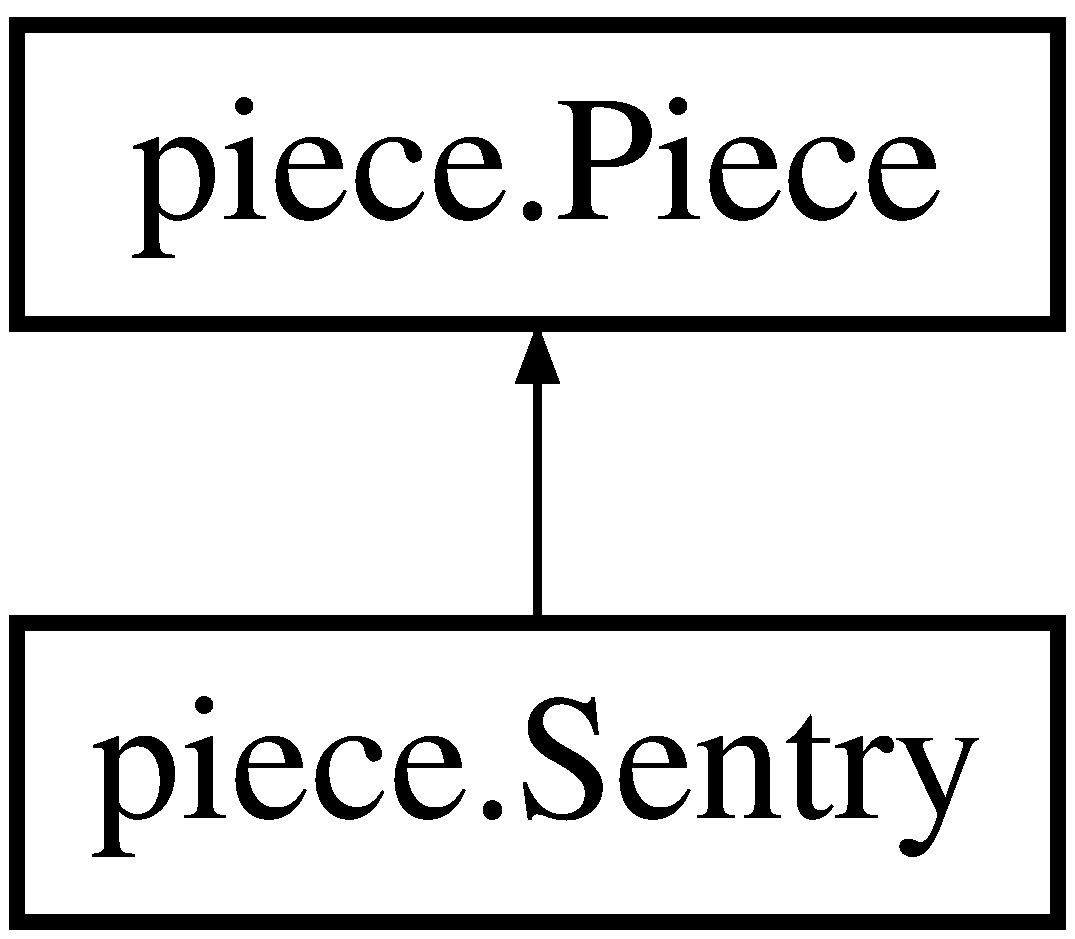
\includegraphics[height=2.000000cm]{classpiece_1_1Sentry}
\end{center}
\end{figure}
\subsection*{Public Member Functions}
\begin{DoxyCompactItemize}
\item 
void \hyperlink{classpiece_1_1Sentry_adfcb33eac6e929b960ad991cd073bf5e}{update\-Moves} (\hyperlink{classmodel_1_1Board}{Board} board)
\end{DoxyCompactItemize}
\subsection*{Additional Inherited Members}


\subsection{Member Function Documentation}
\hypertarget{classpiece_1_1Sentry_adfcb33eac6e929b960ad991cd073bf5e}{\index{piece\-::\-Sentry@{piece\-::\-Sentry}!update\-Moves@{update\-Moves}}
\index{update\-Moves@{update\-Moves}!piece::Sentry@{piece\-::\-Sentry}}
\subsubsection[{update\-Moves}]{\setlength{\rightskip}{0pt plus 5cm}void piece.\-Sentry.\-update\-Moves (
\begin{DoxyParamCaption}
\item[{{\bf Board}}]{board}
\end{DoxyParamCaption}
)\hspace{0.3cm}{\ttfamily [inline]}, {\ttfamily [virtual]}}}\label{classpiece_1_1Sentry_adfcb33eac6e929b960ad991cd073bf5e}
Upates the possible moves for a given piece. 
\begin{DoxyParams}{Parameters}
{\em spaces} & The state of the chess board. \\
\hline
\end{DoxyParams}


Implements \hyperlink{classpiece_1_1Piece_a4dbb3f3506bfc5c4a2015182857d08e0}{piece.\-Piece}.



The documentation for this class was generated from the following file\-:\begin{DoxyCompactItemize}
\item 
piece/Sentry.\-java\end{DoxyCompactItemize}

\hypertarget{classtest_1_1SentryTest}{\section{test.\-Sentry\-Test Class Reference}
\label{classtest_1_1SentryTest}\index{test.\-Sentry\-Test@{test.\-Sentry\-Test}}
}
\subsection*{Public Member Functions}
\begin{DoxyCompactItemize}
\item 
\hypertarget{classtest_1_1SentryTest_afd17ac06614caf962e68f7277e32b522}{void {\bfseries set\-Up} ()  throws Exception }\label{classtest_1_1SentryTest_afd17ac06614caf962e68f7277e32b522}

\item 
\hypertarget{classtest_1_1SentryTest_afa4a4c9d62b3b58ca2bafc64fd4489d8}{void {\bfseries set\-Sentry} ()}\label{classtest_1_1SentryTest_afa4a4c9d62b3b58ca2bafc64fd4489d8}

\item 
\hypertarget{classtest_1_1SentryTest_ada1b84d072bd7ce380d2154e0e9e1711}{void {\bfseries wierd\-Move} ()}\label{classtest_1_1SentryTest_ada1b84d072bd7ce380d2154e0e9e1711}

\item 
\hypertarget{classtest_1_1SentryTest_a49e42f05db2fb533073c833a5415f50c}{void {\bfseries move\-One\-Diagonal} ()}\label{classtest_1_1SentryTest_a49e42f05db2fb533073c833a5415f50c}

\item 
\hypertarget{classtest_1_1SentryTest_a6af984de6d97636f6b58f9119360caa5}{void {\bfseries move\-Two\-Diagonal} ()}\label{classtest_1_1SentryTest_a6af984de6d97636f6b58f9119360caa5}

\item 
\hypertarget{classtest_1_1SentryTest_a3fc2a494dcb45bce4acdfac52fd5e5cb}{void {\bfseries move\-One\-Horizontal} ()}\label{classtest_1_1SentryTest_a3fc2a494dcb45bce4acdfac52fd5e5cb}

\item 
\hypertarget{classtest_1_1SentryTest_a87efc7d365443304d2500c51ed1a996f}{void {\bfseries move\-One\-Vertical} ()}\label{classtest_1_1SentryTest_a87efc7d365443304d2500c51ed1a996f}

\item 
\hypertarget{classtest_1_1SentryTest_a56ed76f2b9c7cd09eeaa73373276669a}{void {\bfseries move\-Two\-Horizontal} ()}\label{classtest_1_1SentryTest_a56ed76f2b9c7cd09eeaa73373276669a}

\item 
\hypertarget{classtest_1_1SentryTest_aac1e64c4a15aa3fc3621a9972eacc95d}{void {\bfseries move\-Two\-Vertical} ()}\label{classtest_1_1SentryTest_aac1e64c4a15aa3fc3621a9972eacc95d}

\end{DoxyCompactItemize}


The documentation for this class was generated from the following file\-:\begin{DoxyCompactItemize}
\item 
test/Sentry\-Test.\-java\end{DoxyCompactItemize}

\hypertarget{classmodel_1_1Space}{\section{model.\-Space Class Reference}
\label{classmodel_1_1Space}\index{model.\-Space@{model.\-Space}}
}
\subsection*{Public Member Functions}
\begin{DoxyCompactItemize}
\item 
\hyperlink{classmodel_1_1Space_a102225bd506d830f347c5f7d24ef11b4}{Space} (int r, int f)
\item 
boolean \hyperlink{classmodel_1_1Space_a3e3cf928913dd8eb206183f17ac1dfb6}{equals} (\hyperlink{classmodel_1_1Space}{Space} other)
\item 
boolean \hyperlink{classmodel_1_1Space_a329bb43b86116fb41e6fdca9cfe818cb}{equals} (int rank, int file)
\item 
int \hyperlink{classmodel_1_1Space_a2104ac93290b6a58994fa548be3207c4}{get\-File} ()
\item 
int \hyperlink{classmodel_1_1Space_a5e09810afbf3d6d9dfd757ec16e0a569}{get\-Rank} ()
\item 
void \hyperlink{classmodel_1_1Space_ad0cf3a2cc956489ec529c9a4aa10d096}{set\-File} (int file)
\item 
void \hyperlink{classmodel_1_1Space_a5a6c913293dc66fe0cf564316dcfc062}{set\-Rank} (int rank)
\end{DoxyCompactItemize}


\subsection{Constructor \& Destructor Documentation}
\hypertarget{classmodel_1_1Space_a102225bd506d830f347c5f7d24ef11b4}{\index{model\-::\-Space@{model\-::\-Space}!Space@{Space}}
\index{Space@{Space}!model::Space@{model\-::\-Space}}
\subsubsection[{Space}]{\setlength{\rightskip}{0pt plus 5cm}model.\-Space.\-Space (
\begin{DoxyParamCaption}
\item[{int}]{r, }
\item[{int}]{f}
\end{DoxyParamCaption}
)\hspace{0.3cm}{\ttfamily [inline]}}}\label{classmodel_1_1Space_a102225bd506d830f347c5f7d24ef11b4}

\begin{DoxyParams}{Parameters}
{\em r} & \\
\hline
{\em f} & \\
\hline
\end{DoxyParams}


\subsection{Member Function Documentation}
\hypertarget{classmodel_1_1Space_a3e3cf928913dd8eb206183f17ac1dfb6}{\index{model\-::\-Space@{model\-::\-Space}!equals@{equals}}
\index{equals@{equals}!model::Space@{model\-::\-Space}}
\subsubsection[{equals}]{\setlength{\rightskip}{0pt plus 5cm}boolean model.\-Space.\-equals (
\begin{DoxyParamCaption}
\item[{{\bf Space}}]{other}
\end{DoxyParamCaption}
)\hspace{0.3cm}{\ttfamily [inline]}}}\label{classmodel_1_1Space_a3e3cf928913dd8eb206183f17ac1dfb6}

\begin{DoxyParams}{Parameters}
{\em other} & \\
\hline
\end{DoxyParams}
\begin{DoxyReturn}{Returns}

\end{DoxyReturn}
\hypertarget{classmodel_1_1Space_a329bb43b86116fb41e6fdca9cfe818cb}{\index{model\-::\-Space@{model\-::\-Space}!equals@{equals}}
\index{equals@{equals}!model::Space@{model\-::\-Space}}
\subsubsection[{equals}]{\setlength{\rightskip}{0pt plus 5cm}boolean model.\-Space.\-equals (
\begin{DoxyParamCaption}
\item[{int}]{rank, }
\item[{int}]{file}
\end{DoxyParamCaption}
)\hspace{0.3cm}{\ttfamily [inline]}}}\label{classmodel_1_1Space_a329bb43b86116fb41e6fdca9cfe818cb}

\begin{DoxyParams}{Parameters}
{\em rank} & \\
\hline
{\em file} & \\
\hline
\end{DoxyParams}
\begin{DoxyReturn}{Returns}
true if the given rank and file values match the space. 
\end{DoxyReturn}
\hypertarget{classmodel_1_1Space_a2104ac93290b6a58994fa548be3207c4}{\index{model\-::\-Space@{model\-::\-Space}!get\-File@{get\-File}}
\index{get\-File@{get\-File}!model::Space@{model\-::\-Space}}
\subsubsection[{get\-File}]{\setlength{\rightskip}{0pt plus 5cm}int model.\-Space.\-get\-File (
\begin{DoxyParamCaption}
{}
\end{DoxyParamCaption}
)\hspace{0.3cm}{\ttfamily [inline]}}}\label{classmodel_1_1Space_a2104ac93290b6a58994fa548be3207c4}
\begin{DoxyReturn}{Returns}
file 
\end{DoxyReturn}
\hypertarget{classmodel_1_1Space_a5e09810afbf3d6d9dfd757ec16e0a569}{\index{model\-::\-Space@{model\-::\-Space}!get\-Rank@{get\-Rank}}
\index{get\-Rank@{get\-Rank}!model::Space@{model\-::\-Space}}
\subsubsection[{get\-Rank}]{\setlength{\rightskip}{0pt plus 5cm}int model.\-Space.\-get\-Rank (
\begin{DoxyParamCaption}
{}
\end{DoxyParamCaption}
)\hspace{0.3cm}{\ttfamily [inline]}}}\label{classmodel_1_1Space_a5e09810afbf3d6d9dfd757ec16e0a569}
\begin{DoxyReturn}{Returns}
rank 
\end{DoxyReturn}
\hypertarget{classmodel_1_1Space_ad0cf3a2cc956489ec529c9a4aa10d096}{\index{model\-::\-Space@{model\-::\-Space}!set\-File@{set\-File}}
\index{set\-File@{set\-File}!model::Space@{model\-::\-Space}}
\subsubsection[{set\-File}]{\setlength{\rightskip}{0pt plus 5cm}void model.\-Space.\-set\-File (
\begin{DoxyParamCaption}
\item[{int}]{file}
\end{DoxyParamCaption}
)\hspace{0.3cm}{\ttfamily [inline]}}}\label{classmodel_1_1Space_ad0cf3a2cc956489ec529c9a4aa10d096}

\begin{DoxyParams}{Parameters}
{\em file} & the file to set \\
\hline
\end{DoxyParams}
\hypertarget{classmodel_1_1Space_a5a6c913293dc66fe0cf564316dcfc062}{\index{model\-::\-Space@{model\-::\-Space}!set\-Rank@{set\-Rank}}
\index{set\-Rank@{set\-Rank}!model::Space@{model\-::\-Space}}
\subsubsection[{set\-Rank}]{\setlength{\rightskip}{0pt plus 5cm}void model.\-Space.\-set\-Rank (
\begin{DoxyParamCaption}
\item[{int}]{rank}
\end{DoxyParamCaption}
)\hspace{0.3cm}{\ttfamily [inline]}}}\label{classmodel_1_1Space_a5a6c913293dc66fe0cf564316dcfc062}

\begin{DoxyParams}{Parameters}
{\em rank} & the rank to set \\
\hline
\end{DoxyParams}


The documentation for this class was generated from the following file\-:\begin{DoxyCompactItemize}
\item 
model/Space.\-java\end{DoxyCompactItemize}

\hypertarget{classcontroller_1_1Step}{\section{controller.\-Step Class Reference}
\label{classcontroller_1_1Step}\index{controller.\-Step@{controller.\-Step}}
}
\subsection*{Public Member Functions}
\begin{DoxyCompactItemize}
\item 
\hyperlink{classcontroller_1_1Step_ab3820dfaff4db43514df302db0bf78ef}{Step} (int rank\-\_\-i, int file\-\_\-i, int rank\-\_\-f, int file\-\_\-f, \hyperlink{classpiece_1_1Piece}{Piece} eaten\-Piece)
\end{DoxyCompactItemize}
\subsection*{Public Attributes}
\begin{DoxyCompactItemize}
\item 
\hypertarget{classcontroller_1_1Step_ac96c44339141074bf3c11802bc863a41}{int {\bfseries rank\-\_\-i}}\label{classcontroller_1_1Step_ac96c44339141074bf3c11802bc863a41}

\item 
\hypertarget{classcontroller_1_1Step_ae9c6ee95f3b4afa6c54240a7854da92b}{int {\bfseries file\-\_\-i}}\label{classcontroller_1_1Step_ae9c6ee95f3b4afa6c54240a7854da92b}

\item 
\hypertarget{classcontroller_1_1Step_af5900d1d354170b6294ca8040b334d87}{int {\bfseries rank\-\_\-f}}\label{classcontroller_1_1Step_af5900d1d354170b6294ca8040b334d87}

\item 
\hypertarget{classcontroller_1_1Step_aa0b5dab8a2fd16aa91fccfd7598f18d3}{int {\bfseries file\-\_\-f}}\label{classcontroller_1_1Step_aa0b5dab8a2fd16aa91fccfd7598f18d3}

\item 
\hypertarget{classcontroller_1_1Step_a6b919a98e7a389b561a0cfb010a3f41c}{\hyperlink{classpiece_1_1Piece}{Piece} {\bfseries eaten\-Piece}}\label{classcontroller_1_1Step_a6b919a98e7a389b561a0cfb010a3f41c}

\end{DoxyCompactItemize}


\subsection{Constructor \& Destructor Documentation}
\hypertarget{classcontroller_1_1Step_ab3820dfaff4db43514df302db0bf78ef}{\index{controller\-::\-Step@{controller\-::\-Step}!Step@{Step}}
\index{Step@{Step}!controller::Step@{controller\-::\-Step}}
\subsubsection[{Step}]{\setlength{\rightskip}{0pt plus 5cm}controller.\-Step.\-Step (
\begin{DoxyParamCaption}
\item[{int}]{rank\-\_\-i, }
\item[{int}]{file\-\_\-i, }
\item[{int}]{rank\-\_\-f, }
\item[{int}]{file\-\_\-f, }
\item[{{\bf Piece}}]{eaten\-Piece}
\end{DoxyParamCaption}
)\hspace{0.3cm}{\ttfamily [inline]}}}\label{classcontroller_1_1Step_ab3820dfaff4db43514df302db0bf78ef}

\begin{DoxyParams}{Parameters}
{\em rank\-\_\-i} & \\
\hline
{\em file\-\_\-i} & \\
\hline
{\em rank\-\_\-f} & \\
\hline
{\em file\-\_\-f} & \\
\hline
{\em eaten\-Piece} & \\
\hline
\end{DoxyParams}


The documentation for this class was generated from the following file\-:\begin{DoxyCompactItemize}
\item 
controller/Step.\-java\end{DoxyCompactItemize}

\addcontentsline{toc}{part}{Index}
\printindex
\end{document}
